\documentclass[12pt,a4paper]{report}

% Page geometry and layout
\usepackage[margin=2.5cm, headheight=28pt]{geometry}

% Professional headers and footers
\usepackage{fancyhdr}
\pagestyle{fancy}
\setlength{\headheight}{28pt}
\fancyhf{}
\fancyhead[L]{\leftmark}
\fancyhead[R]{\thepage}
\renewcommand{\headrulewidth}{0.4pt}

% Enhanced title formatting
\usepackage{titlesec}
\titleformat{\chapter}[display]
  {\normalfont\huge\bfseries}{\chaptertitlename\ \thechapter}{20pt}{\Huge}
\titlespacing*{\chapter}{0pt}{-20pt}{40pt}

% Table of contents enhancements
\usepackage{tocbibind}
\setcounter{tocdepth}{3}
\setcounter{secnumdepth}{3}

% Graphics and diagrams
\usepackage{graphicx}
\usepackage{float}
\usepackage{tikz}
\usetikzlibrary{positioning,shapes.geometric,arrows.meta}
\usepackage{pgfplots}
\pgfplotsset{compat=1.18}

% Additional packages for academic writing
\usepackage{amsmath}
\usepackage{amssymb}
\usepackage{enumitem}
\usepackage{listings}
\usepackage{xcolor}
\usepackage{url}
\usepackage{footnote}
\usepackage{subcaption}
\usepackage{pgf-umlsd}
\usepackage{pdfpages}

% Code formatting for environments migrated from minted to listings
\lstset{
  basicstyle=\ttfamily\footnotesize,
  breaklines=true,
  columns=fullflexible,
  keepspaces=true,
  frame=single,
  showstringspaces=false,
  tabsize=2
}

% Shared TikZ styles used across chapter diagrams
\tikzset{
  actor/.style={ellipse, draw, minimum width=2.2cm, minimum height=0.9cm, align=center},
  system/.style={rectangle, draw, thick, rounded corners, minimum width=3.2cm, minimum height=1.1cm, align=center},
  usecase/.style={ellipse, draw, minimum width=2.4cm, minimum height=1.0cm, align=center},
  entity/.style={rectangle, draw, rounded corners, minimum width=2.4cm, minimum height=0.9cm, align=center},
  relationship/.style={diamond, draw, aspect=1.6, minimum width=1.8cm, align=center},
  umlclass/.style={rectangle, draw, rounded corners, minimum width=4.0cm, minimum height=1.2cm, align=left, font=\small\ttfamily, inner sep=4pt},
  state/.style={rectangle, draw, rounded corners, minimum width=2.2cm, minimum height=0.8cm, align=center}
}

% Enhanced tables
\usepackage{booktabs}
\usepackage{tabularx}
\usepackage{multirow}

% Hyperlinks and cross-references
\usepackage[pdftex,
  colorlinks=true,
  linkcolor=blue,
  citecolor=blue,
  urlcolor=blue,
  pdftitle={RM - Report Manager: Web and Mobile Application for IT Equipment Installation Management},
  pdfauthor={Your Name},
  pdfsubject={Master's Final Year Engineering Project},
  pdfkeywords={Spring Boot, JHipster, Angular, Flutter, PostgreSQL, Docker, SCRUM}
]{hyperref}
\usepackage{cleveref}

% Custom commands for consistent formatting
\newcommand{\code}[1]{\texttt{#1}}
\newcommand{\api}[1]{\texttt{/api/#1}}
\newcommand{\entity}[1]{\textit{#1}}
\newcommand{\usecase}[1]{\textbf{UC-#1}}

\begin{document}

\includepdf[pages=-]{garde_organized.pdf}

% Title page

% Abstract
\cleardoublepage
\thispagestyle{empty}

\begin{center}

{\Large\textit{DEDICATION}}

\vspace{1cm}

\textbf{To my dear family,}

\vspace{0.3cm}

I dedicate this work to you, whose unconditional love, sacrifices, and unwavering support have shaped who I am today.
You have been my strength in difficult times and my joy in moments of success.
Your guidance, patience, and encouragement have allowed me to move forward with confidence and determination.
This achievement carries a part of each of you, and I hope it reflects my deepest gratitude and makes you proud.
\vspace{0.6cm}

\textbf{To my closest friends --- EL ``Cliqua'',}

\vspace{0.3cm}

Calling you simply friends would be an understatement.  
You are a second family who have filled my life with unforgettable memories, laughter, and support.  
Through the ups and downs of this journey, your presence made every challenge easier and every success more meaningful.  
Thank you for the encouragement, the motivation, and the countless moments that made these years truly special.  
This work is also yours.

\vspace{0.6cm}

\textbf{To Faten,}

\vspace{0.3cm}

Your pure soul and kind heart have always been a safe space where I can truly be myself.  
You have a unique way of making me believe in myself and see things with more clarity and confidence.  
Your presence in my life brings calm, balance, and a steadiness that helps me move forward with a clearer vision.  
For the inner peace and strength you bring into my life, I dedicate this work to you with sincere affection.

\vspace{0.8cm}

\textit{With gratitude and love}

\end{center}

\cleardoublepage

\cleardoublepage
\thispagestyle{empty}

\begin{center}

{\Large\textit{ACKNOWLEDGEMENTS}}

\vspace{1cm}

\textbf{First and foremost, to God,}

\vspace{0.3cm}

I would like to express my deepest gratitude to God for granting me the strength, patience, and perseverance needed to complete this work.  
Throughout this journey, His guidance has helped me overcome challenges and continue moving forward with determination.  
Without these blessings, the completion of this project would not have been possible.

\vspace{0.6cm}

\textbf{To my academic supervisor Maroua BELKNENI,}

\vspace{0.3cm}

I would like to express my sincere appreciation to my academic supervisor for their guidance, valuable advice, and continuous support throughout the realization of this project.  
Their insights and encouragement played an essential role in shaping this work and helping me overcome many challenges during this journey.

\vspace{0.6cm}

\textbf{To my professional supervisor Nader KESSENTINI,}

\vspace{0.3cm}

I would like to extend my sincere thanks to my professional supervisor for giving me the opportunity to carry out my final year project within the company.  
Their trust, availability, and practical guidance allowed me to better understand the professional environment and apply my academic knowledge to real-world challenges.

\vspace{0.6cm}

\textbf{To the team at Africom Services,}

\vspace{0.3cm}

I would also like to warmly thank the entire team at \textbf{Africom Services} for their welcome, collaboration, and willingness to share their knowledge.  
Working alongside such a supportive and professional team made this experience both enriching and inspiring, and it contributed greatly to my personal and professional growth.

\vspace{0.8cm}

\textit{My sincere gratitude to everyone who contributed, directly or indirectly, to the realization of this work.}

\end{center}

\cleardoublepage

% Table of contents
\tableofcontents

% List of figures
\listoffigures

% List of tables
\listoftables

% General Introduction
% \chapter*{General Introduction}
\addcontentsline{toc}{chapter}{General Introduction}

\section{Context of the Internship and Project}

This final-year engineering project was carried out at Africom Services, a Tunisian company founded in January 2005 by experienced telecommunications executives. The company operates in telecommunications engineering and network maintenance, with activities covering transmission systems, radio-electric networks, fiber-optic deployment, electronic security, and integrated energy/IT solutions.

Africom Services supports telecom operators, private companies, and public institutions in modernizing communication infrastructure. Its technical positioning is reinforced by a collaboration with Telecom Canada, which provides additional expertise in private networks, wireless communication, and digital infrastructure.

Within this context, the company identified a recurring operational challenge in field intervention management: intervention data were often captured through fragmented and partially manual workflows, making monitoring, validation, and reporting slower and less reliable than required for modern service delivery.

\section{Problem Statement and Motivation}

The management of IT equipment installation and maintenance interventions involves multiple stakeholders, distributed teams, and strict quality constraints. In practice, the existing process generated five major limitations:

\begin{enumerate}
\item Delays between intervention execution and report delivery.
\item Heterogeneous data capture quality across technicians and projects.
\item Limited real-time visibility for supervisors and coordinators.
\item Difficulty in enforcing standardized workflows and validation rules.
\item Administrative overhead in consolidating intervention outputs for clients.
\end{enumerate}

These limitations motivated the design of an integrated digital platform able to structure the complete intervention lifecycle from planning to execution, validation, and reporting.

\section{Project Objective}

The objective of this project is to design and implement \textbf{RM (Report Manager)}, a web and mobile solution dedicated to intervention management for IT equipment installation and maintenance activities.

The project pursues the following specific objectives:

\begin{itemize}
\item Digitize and standardize intervention workflows.
\item Enable role-based collaboration between technicians, supervisors, coordinators, and administrators.
\item Improve traceability through status control, audit information, and structured evidence management.
\item Automate the production of operational reports for decision-making and client communication.
\item Provide a scalable technical foundation aligned with industrial software engineering practices.
\end{itemize}

\section{Methodological Approach}

The project follows an agile SCRUM process based on incremental delivery. Development was organized into iterative sprints, each targeting a coherent functional scope and ending with validation activities.

This methodology was selected to:

\begin{itemize}
\item maintain continuous alignment with operational needs,
\item reduce technical and organizational risk through progressive delivery,
\item and integrate feedback loops for quality improvement.
\end{itemize}

In practical execution, the SCRUM framework was adapted to a single-developer delivery model with explicit control of backlog prioritization, sprint planning, and sprint review checkpoints. This adaptation preserved methodological rigor while remaining compatible with academic time constraints.

From a technical perspective, the implementation combines a backend service layer, a web interface, and a mobile client, supported by a secure and structured data management strategy.

\section{Report Organization}

The remainder of this report is organized as follows:

\begin{itemize}
\item \textbf{Chapter 1: General Presentation} introduces the host company, project environment, problematic, and objectives.
\item \textbf{Chapter 2: Project Planning} presents the SCRUM process, tools, and physical/logical architecture decisions.
\item \textbf{Chapter 3: Analysis and Requirements Specification} formalizes actors, role codes, functional and non-functional requirements, use cases, and backlog structure.
\item \textbf{Chapter 4: Sprint 1} details foundation and core infrastructure implementation.
\item \textbf{Chapter 5: Sprint 2} presents rapport request and dynamic form template realization.
\item \textbf{Chapter 6: Sprint 3} covers file management and geolocation tracking features.
\item \textbf{Chapter 7: Sprint 4} documents approval workflow, rejection logic, and status governance.
\item \textbf{Chapter 8: Sprint 5} presents reporting, export integration, and optimization mechanisms.
\item \textbf{General Conclusion} synthesizes achievements, limitations, and future work perspectives.
\end{itemize}

This structure ensures a coherent progression from contextual framing and requirement formalization to design rationale, implementation details, and critical evaluation of results.


% Chapter 1: General Presentation
\chapter{General Presentation}

\section{Introduction}

This chapter establishes the strategic and operational framing of the project. It presents the general framework, introduces the host organization, details project background and problematic, and studies the existing intervention management process to justify the proposed digital solution.

\section{General Framework of the Project}

The RM project belongs to the digital transformation of field operations in telecom and IT equipment installation contexts. In such environments, intervention quality depends on rapid coordination between office teams and field technicians, consistent data collection, and reliable validation cycles.

From a systems engineering perspective, this context imposes five structural constraints:

\begin{enumerate}
\item distributed operations across multiple sites,
\item heterogeneous intervention scenarios requiring configurable forms,
\item strict accountability expectations from clients and operators,
\item tight turnaround targets for validation and reporting,
\item and high dependence on mobile data capture under variable connectivity.
\end{enumerate}

Consequently, the project is not only a software implementation effort. It is also a process reengineering initiative where workflow governance, traceability, and data quality control are central design objectives.

\section{Presentation of the Host Organization}

\subsection{Organizational Identity}

Africom Services is a Tunisian company founded in 2005 and active in telecommunications engineering, field deployment, and maintenance services. The organization supports telecom operators, enterprise clients, and institutional actors through project execution and technical operations.

\subsection{Core Activity Areas}

\begin{itemize}
\item deployment and validation of telecom transmission equipment,
\item radio network and microwave infrastructure projects,
\item fiber optic implementation and maintenance,
\item preventive and corrective technical interventions,
\item operational monitoring solutions and connected security services.
\end{itemize}

\subsection{Operational Characteristics}

The organization combines office-based coordination with field execution teams. This dual operating model creates strong demand for synchronized information systems able to connect planning, execution evidence, quality control, and reporting.

\begin{figure}[H]
\centering
\fbox{\parbox{0.88\textwidth}{
\centering
% TODO: Insert host organization chart here
Organization Chart Placeholder: Operational management, coordination unit, supervision unit, field technician teams.
}}
\caption{Host Organization Structure Placeholder}
\label{fig:host_org_structure_placeholder}
\end{figure}

\section{Project Presentation}

\subsection{Project Background}

Before RM, intervention governance relied on partially fragmented practices with heterogeneous tools and significant manual effort. The operational flow from assignment to final report delivery lacked a unified digital backbone. As intervention volume increased, this model exposed scalability limits.

The PRD therefore defined RM as an integrated web and mobile platform with the following business mission:

\begin{itemize}
\item standardize intervention execution through template-driven processes,
\item improve supervisor visibility on field progress,
\item enforce validation and rejection governance,
\item and automate client-ready Excel reporting.
\end{itemize}

\subsection{Problematic}

The project problematic can be formalized as:

\begin{quote}
How can a telecom field-operations organization move from fragmented, partly manual intervention tracking to a controlled, auditable, and scalable digital workflow without reducing field agility?
\end{quote}

This problematic combines business and technical dimensions:

\begin{itemize}
\item business dimension: cycle time reduction, quality consistency, and managerial visibility,
\item technical dimension: secure multi-platform architecture, dynamic form support, and robust traceability.
\end{itemize}

\section{Study of the Existent}

\subsection{Analysis of the Existing}

The initial process can be summarized in six stages:

\begin{enumerate}
\item request preparation by coordination staff,
\item technician assignment through ad-hoc communication,
\item field execution and evidence collection,
\item supervisor quality checks,
\item correction loop when errors are detected,
\item final report consolidation for client communication.
\end{enumerate}

Observed process weaknesses were concentrated at handoff points between stakeholders, where information loss and delay frequently occurred.

\begin{table}[H]
\centering
\caption{Observed Weaknesses in the Existing Process}
\label{tab:existing_process_weaknesses}
\begin{tabularx}{\textwidth}{|l|X|X|}
\hline
\textbf{Process Stage} & \textbf{Observed Issue} & \textbf{Operational Impact} \\
\hline
Assignment and planning & Inconsistent data format between teams & Rework and interpretation errors \\
\hline
Field execution & Non-standardized capture structure & Data quality variability \\
\hline
Validation & Limited immediate access to complete evidence & Longer decision cycle time \\
\hline
Reporting & Manual consolidation effort & Delayed delivery and reduced scalability \\
\hline
Audit and compliance & Partial history tracking & Difficult incident analysis and accountability \\
\hline
\end{tabularx}
\end{table}

\subsection{Critique of the Existing}

The existing process can be critiqued using a quality-attribute lens:

\begin{itemize}
\item \textbf{Traceability deficit}: status transitions and decision rationale were not uniformly logged.
\item \textbf{Standardization deficit}: different technicians used different capture practices.
\item \textbf{Responsiveness deficit}: supervisors had delayed visibility on field outputs.
\item \textbf{Scalability deficit}: manual aggregation could not scale with intervention growth.
\item \textbf{Governance deficit}: control rules were implicit rather than encoded in system behavior.
\end{itemize}

Industry comparison confirms that modern field-service platforms prioritize event-driven status management, structured evidence collection, and automated report generation. The existing model did not provide these capabilities in an integrated way.

\subsection{Proposed Solution}

RM addresses the identified deficits through a domain-driven digital platform organized around five pillars:

\begin{enumerate}
\item \textbf{Identity and governance}: JWT authentication with role-based control.
\item \textbf{Workflow control}: lifecycle management from planning to approval and archival.
\item \textbf{Template-driven execution}: dynamic forms for standardized field data capture.
\item \textbf{Evidence and traceability}: files, geolocation, and status history.
\item \textbf{Automated reporting}: configurable Excel generation aligned with operator needs.
\end{enumerate}

\begin{figure}[H]
\centering
\fbox{\parbox{0.9\textwidth}{
\centering
% TODO: Insert as-is vs to-be process diagram here
Process Transformation Placeholder: Existing fragmented flow versus RM integrated digital workflow.
}}
\caption{As-Is and To-Be Process Comparison Placeholder}
\label{fig:as_is_to_be_placeholder}
\end{figure}

\section{Conclusion}

This chapter provided the business and organizational grounding of the RM project. It demonstrated why the legacy process was insufficient for current operational demands and justified the need for a structured digital platform. The next chapter presents the planning approach, tools, and architecture decisions used to operationalize this transformation.


% Chapter 2: Analysis and Requirements Specification
\chapter{Analysis and Requirements Specification}

\section{Introduction}

This chapter formalizes the analysis phase of the RM project. It identifies system actors, specifies functional and non-functional requirements, models principal use cases, and states the project constraints that shape design and implementation decisions.

\section{Stakeholder and Actor Analysis}

\subsection{Primary Actors}

\begin{itemize}
\item \textbf{Technician}: executes interventions in the field, fills forms, attaches evidence, and updates intervention status.
\item \textbf{Supervisor}: assigns interventions, verifies execution quality, and approves or rejects completed interventions.
\item \textbf{Coordinator}: creates intervention requests, configures templates, and generates management reports.
\item \textbf{Administrator}: manages users, roles, and global system configuration.
\end{itemize}

\subsection{Secondary Stakeholders}

\begin{itemize}
\item \textbf{Client organizations}: receive validated intervention reports.
\item \textbf{Operational management}: monitors performance indicators and service quality.
\item \textbf{Technical support}: ensures platform continuity and incident resolution.
\end{itemize}

\section{Roles and Access Control}

The platform applies role-based access control (RBAC) to ensure secure and traceable operations.

\begin{table}[H]
\centering
\caption{Roles and Permissions Matrix}
\label{tab:roles_permissions_reworked}
\begin{tabularx}{\textwidth}{|l|X|X|X|X|}
\hline
\textbf{Permission} & \textbf{Technician} & \textbf{Supervisor} & \textbf{Coordinator} & \textbf{Administrator} \\
\hline
View assigned interventions & \checkmark & \checkmark & \checkmark & \checkmark \\
\hline
Update intervention status & \checkmark & \checkmark & \checkmark & \checkmark \\
\hline
Complete intervention forms & \checkmark & \checkmark & \checkmark & \checkmark \\
\hline
Assign interventions & & \checkmark & \checkmark & \checkmark \\
\hline
Approve interventions & & \checkmark & \checkmark & \checkmark \\
\hline
Create intervention requests & & & \checkmark & \checkmark \\
\hline
Configure templates & & & \checkmark & \checkmark \\
\hline
Generate reports & & & \checkmark & \checkmark \\
\hline
Manage users and roles & & & & \checkmark \\
\hline
System configuration & & & & \checkmark \\
\hline
\end{tabularx}
\end{table}

\section{Functional Requirements}

Functional requirements are grouped by capability domain.

\subsection{Authentication and Security}

\begin{enumerate}
\item The system shall authenticate users with secure credentials.
\item The system shall maintain authenticated sessions using token-based authorization.
\item The system shall enforce access control according to user roles.
\item The system shall maintain audit information on critical operations.
\end{enumerate}

\subsection{Intervention Lifecycle Management}

\begin{enumerate}
\item The system shall allow creation of intervention requests based on predefined templates.
\item The system shall support assignment of interventions to technicians.
\item The system shall support lifecycle status transitions from planning to archival.
\item The system shall allow supervisors to approve or reject intervention submissions.
\item The system shall keep a history of status changes and comments.
\end{enumerate}

\subsection{Template and Dynamic Form Management}

\begin{enumerate}
\item The system shall allow coordinators to create and manage reusable form templates.
\item The system shall generate intervention forms dynamically from selected templates.
\item The system shall validate required fields and form consistency before submission.
\end{enumerate}

\subsection{Evidence and Document Management}

\begin{enumerate}
\item The system shall allow upload and download of intervention-related files.
\item The system shall associate evidence files with interventions and users.
\item The system shall preserve file metadata for traceability.
\end{enumerate}

\subsection{Reporting and Monitoring}

\begin{enumerate}
\item The system shall generate report outputs for operational and managerial use.
\item The system shall support filtered views by project, status, and date.
\item The system shall provide dashboard information for supervision and follow-up.
\end{enumerate}

\section{Non-Functional Requirements}

\subsection{Performance}

\begin{itemize}
\item Response times should remain acceptable under concurrent usage.
\item Report generation and file operations should be optimized for operational workload.
\end{itemize}

\subsection{Reliability and Availability}

\begin{itemize}
\item The platform must ensure data persistence and recovery mechanisms.
\item Operational continuity must be maintained during normal business activity.
\end{itemize}

\subsection{Security}

\begin{itemize}
\item Authentication and authorization must protect sensitive operational data.
\item Input validation must reduce injection and data integrity risks.
\item Access to evidence and reports must be controlled by roles and permissions.
\end{itemize}

\subsection{Usability}

\begin{itemize}
\item Interfaces should remain clear for both office and field users.
\item Mobile workflows should support quick intervention data capture.
\end{itemize}

\subsection{Maintainability and Scalability}

\begin{itemize}
\item Architecture and code organization should support incremental evolution.
\item The platform should accommodate additional modules and reporting needs.
\end{itemize}

\section{System Use Cases}

\subsection{Core Use Cases by Actor}

\begin{table}[H]
\centering
\caption{Main Use Cases by Actor}
\label{tab:use_cases_by_actor}
\begin{tabularx}{\textwidth}{|l|X|}
\hline
\textbf{Actor} & \textbf{Main Use Cases} \\
\hline
Technician & Consult assigned intervention, complete dynamic form, upload evidence, submit execution output \\
\hline
Supervisor & Assign intervention, review submission, approve or reject with feedback, monitor pending items \\
\hline
Coordinator & Create intervention request, manage templates, track project progress, generate reports \\
\hline
Administrator & Manage users and roles, configure system parameters, supervise platform health \\
\hline
\end{tabularx}
\end{table}

\subsection{Representative Use Case: Intervention Validation}

\textbf{Primary actor:} Supervisor

\textbf{Preconditions:}
\begin{itemize}
\item A technician has submitted intervention data.
\item Required form fields and evidence are available.
\end{itemize}

\textbf{Main scenario:}
\begin{enumerate}
\item Supervisor opens the pending intervention.
\item Supervisor reviews captured values and attachments.
\item Supervisor either approves the intervention or rejects it with feedback.
\item System updates status history and notifies relevant actors.
\end{enumerate}

\textbf{Postconditions:}
\begin{itemize}
\item Intervention status is updated and traceable.
\item Follow-up actions become available according to the new state.
\end{itemize}

\section{Project Constraints}

\begin{itemize}
\item \textbf{Time constraint}: development and validation were performed within an academic calendar.
\item \textbf{Organizational constraint}: workflows had to align with existing operational practices.
\item \textbf{Technical constraint}: integration had to remain compatible with selected stack components and deployment model.
\item \textbf{Data constraint}: intervention data and evidence require controlled access and structured storage.
\item \textbf{Quality constraint}: solution acceptance depends on traceability, consistency, and report reliability.
\end{itemize}

\section{Chapter Conclusion}

This chapter transformed operational needs into formal requirements and constraints. It established the functional perimeter of the system and defined the quality criteria that guide architecture and implementation. The next chapter presents the design decisions adopted to satisfy these requirements.


% Chapter 3: System Design
\chapter{System Design}

\section{Introduction}

This chapter presents the design choices retained for RM. It covers architectural principles, logical decomposition, data design, workflow modeling, and interface structuring. The objective is to show how the design responds directly to the requirements defined in Chapter 2.

\section{Design Principles}

The design is guided by five principles:

\begin{enumerate}
\item \textbf{Separation of concerns}: clear distinction between business logic, data access, and presentation layers.
\item \textbf{Traceability}: explicit status transitions and historical records for intervention follow-up.
\item \textbf{Configurability}: template-based forms to support heterogeneous intervention scenarios.
\item \textbf{Security by design}: role-aware access and controlled data exposure.
\item \textbf{Scalability}: modular components that can evolve with organizational growth.
\end{enumerate}

\section{Global Architecture}

\subsection{Physical and Deployment View}

The system is organized around a web client, a mobile client, and backend services connected to persistent storage. This deployment supports office workflows and field operations simultaneously.

\begin{itemize}
\item \textbf{Web layer}: supervision, request creation, template configuration, and reporting.
\item \textbf{Mobile layer}: field execution, dynamic form completion, evidence capture.
\item \textbf{Backend layer}: authentication, intervention lifecycle services, reporting services.
\item \textbf{Data layer}: structured entities and dynamic payload storage.
\end{itemize}

\subsection{Logical View}

The logical decomposition follows domain-oriented modules:

\begin{enumerate}
\item Identity and access management
\item Intervention and status management
\item Template and dynamic form management
\item Evidence and file management
\item Reporting and monitoring
\end{enumerate}

\section{Domain and Data Design}

\subsection{Core Domain Entities}

The conceptual domain includes the following core entities:

\begin{itemize}
\item \textbf{User} and \textbf{Role}: identity and authorization model.
\item \textbf{Project} and \textbf{Client}: organizational context of interventions.
\item \textbf{Template}: reusable form structure and validation rules.
\item \textbf{Intervention Request}: operational unit assigned for execution.
\item \textbf{Intervention Status History}: lifecycle traceability.
\item \textbf{Attachment}: evidence files linked to interventions.
\end{itemize}

\subsection{Data Modeling Strategy}

A hybrid data model is retained:

\begin{itemize}
\item relational entities for stable business objects,
\item structured dynamic payloads for template-driven intervention data.
\end{itemize}

This strategy balances consistency for core operations and flexibility for evolving field forms.

\section{Process and Workflow Design}

\subsection{Intervention Lifecycle Model}

The intervention lifecycle is designed as a controlled state machine:

\begin{center}
PLANNED $\rightarrow$ EXECUTED $\rightarrow$ PENDING\_VALIDATION $\rightarrow$ APPROVED $\rightarrow$ ARCHIVED
\end{center}

Rejected interventions are redirected to a correction loop before resubmission. This model ensures quality gates while preserving operational fluidity.

\subsection{Approval Workflow}

The approval process formalizes quality control responsibilities:

\begin{enumerate}
\item Technician submits completed intervention.
\item Supervisor reviews form values and evidence.
\item Supervisor approves or rejects with explicit feedback.
\item System records transition and notifies stakeholders.
\end{enumerate}

\section{Use Case Realization Design}

\subsection{Representative Realization: Dynamic Intervention Execution}

The design of dynamic execution follows the sequence below:

\begin{enumerate}
\item Coordinator configures a template.
\item Supervisor creates an intervention request based on that template.
\item Technician receives assignment and opens generated form.
\item Technician captures required values and attachments.
\item Submission triggers validation and status update.
\end{enumerate}

This realization links requirement-level use cases to concrete service interactions.

\section{Interface Design}

\subsection{Web Interface Design}

The web interface is designed around role-driven dashboards:

\begin{itemize}
\item coordinator workspace for planning and template management,
\item supervisor workspace for assignment and validation,
\item administration workspace for configuration and governance.
\end{itemize}

\subsection{Mobile Interface Design}

The mobile interface prioritizes field usability:

\begin{itemize}
\item fast intervention access,
\item guided dynamic form completion,
\item evidence capture,
\item resilient behavior under unstable connectivity conditions.
\end{itemize}

\section{Design Validation Against Requirements}

The proposed design satisfies key requirement families:

\begin{itemize}
\item \textbf{Functional fit}: complete coverage of intervention, template, validation, and reporting flows.
\item \textbf{Security fit}: role-centered access and controlled operations.
\item \textbf{Performance fit}: modular decomposition and efficient data access paths.
\item \textbf{Maintainability fit}: clear architecture boundaries and extensible modules.
\end{itemize}

\section{Chapter Conclusion}

This chapter established the architectural and modeling foundation of RM. It demonstrated how requirements were translated into a coherent system structure. The next chapter details the implementation strategy and the realization of key modules.


% Chapter 4: Implementation
\chapter{Implementation}

\section{Introduction}

This chapter presents the technical realization of RM. It describes implementation choices for backend services, web and mobile interfaces, workflow modules, and reporting capabilities. The objective is to show how design artifacts were translated into a working system.

\section{Implementation Environment}

\subsection{Method and Incremental Delivery}

Implementation followed iterative increments aligned with agile sprint planning. Technical progress moved from foundational infrastructure to advanced operational features.

\subsection{Technology Stack}

\begin{itemize}
\item \textbf{Backend}: Spring Boot ecosystem for service logic and API exposure.
\item \textbf{Data}: PostgreSQL for persistent storage.
\item \textbf{Web frontend}: Angular-based interface for management workflows.
\item \textbf{Mobile frontend}: Flutter client for field operations.
\item \textbf{Deployment support}: containerized runtime and environment isolation.
\end{itemize}

\section{Backend Realization}

\subsection{Security and Access Layer}

The backend implements authenticated access and role-based authorization. Core mechanisms include secure identity validation, controlled endpoint exposure, and permission checks by user role.

\subsection{Domain Services}

Implementation is structured around domain services:

\begin{enumerate}
\item \textbf{Template service}: creation, update, and lifecycle of reusable form templates.
\item \textbf{Intervention service}: request creation, assignment, execution submission, and status transition management.
\item \textbf{Validation service}: approval and rejection logic with traceable feedback.
\item \textbf{Attachment service}: evidence storage and retrieval linked to interventions.
\item \textbf{Reporting service}: extraction and formatting of operational outputs.
\end{enumerate}

\subsection{Persistence and Data Access}

The persistence layer combines stable relational entities and flexible form payload structures. Repository and service abstractions isolate data access concerns and improve maintainability.

\section{Web Application Realization}

\subsection{Coordinator Features}

Implemented coordinator capabilities include:

\begin{itemize}
\item creation and management of intervention requests,
\item template definition and updates,
\item consultation of intervention progress,
\item report launch and export workflows.
\end{itemize}

\subsection{Supervisor Features}

Implemented supervisor capabilities include:

\begin{itemize}
\item intervention assignment to technicians,
\item pending-validation monitoring,
\item approval/rejection actions with comments,
\item visibility over status progression.
\end{itemize}

\subsection{Administrator Features}

The administration scope includes user-role governance and configuration-level controls supporting platform reliability and secure operation.

\section{Mobile Application Realization}

\subsection{Field Execution Workflow}

The mobile client supports the full field cycle:

\begin{enumerate}
\item retrieve assigned intervention,
\item open dynamic form generated from template,
\item capture required values,
\item attach photos/documents,
\item submit execution output for validation.
\end{enumerate}

\subsection{Evidence Capture and Synchronization}

Mobile implementation provides evidence handling with controlled upload behavior and synchronization support adapted to variable network conditions.

\section{Cross-Module Integration}

\subsection{Status and Traceability}

A shared status model ensures consistency between web and mobile channels. Every critical transition is logged with actor and time information for auditability.

\subsection{Notification and Collaboration Flow}

Status-driven notifications support coordination between technicians, supervisors, and coordinators. This reduces processing latency between execution and validation stages.

\section{Implementation by Major Functional Blocks}

\subsection{Block A: Foundation Services}

Delivered components include project infrastructure, identity management, and core domain setup.

\subsection{Block B: Intervention and Template Core}

Delivered components include request management, template-driven forms, and assignment workflows.

\subsection{Block C: Evidence and Validation Enhancements}

Delivered components include file management, workflow validation, and status governance.

\subsection{Block D: Reporting and Optimization Extensions}

Delivered components include report generation features and operational optimization mechanisms.

\section{Chapter Conclusion}

This chapter detailed the implementation of RM across backend, web, and mobile dimensions, with integration mechanisms that ensure coherent operation. The next chapter evaluates obtained results and discusses system performance, value, and limitations.


% Chapter 5: Sprint 2
\chapter{Sprint 2: Rapport Request and Form Templates}

\section{Introduction}

Sprint 2 implemented the first business-critical capabilities of RM by introducing intervention request management and dynamic form template governance. This sprint transformed the platform from an authenticated infrastructure into an operational system that can create, assign, and process intervention activities with structured data capture.

The sprint objective was to digitize the intervention initiation process and standardize data collection through configurable templates.

\section{Preview of Sprint}

\subsection{Sprint Objectives}

\begin{enumerate}
\item Implement intervention request lifecycle creation and assignment.
\item Implement rapport template management with JSON mapping definitions.
\item Build dynamic form generation rules from template configuration.
\item Enforce validation constraints for reliable and consistent submissions.
\item Expose API contracts for web and mobile interaction with intervention data.
\end{enumerate}

\subsection{Business Value Statement}

This sprint addresses the PRD objective of replacing fragmented request processes with a structured digital workflow. It provides standardized form definitions, reducing ambiguity and improving data quality before validation and reporting phases.

\section{Sprint Backlog}

\begin{table}[H]
\centering
\caption{Sprint 2 Backlog}
\label{tab:sprint2_backlog}
\begin{tabularx}{\textwidth}{|l|X|l|l|}
\hline
\textbf{ID} & \textbf{User Story} & \textbf{Points} & \textbf{Status} \\
\hline
S2-1 & Create and assign rapport requests to technicians & 13 & Completed \\
\hline
S2-2 & Configure and maintain rapport templates & 8 & Completed \\
\hline
S2-3 & Generate dynamic forms from template mappings & 8 & Completed \\
\hline
S2-4 & Validate input data and enforce required fields & 8 & Completed \\
\hline
S2-5 & Support request filtering and lookup in web interface & 8 & Completed \\
\hline
\textbf{Total} & & \textbf{45} & \\
\hline
\end{tabularx}
\end{table}

\section{Functional Specifications}

\subsection{Detailed Use Cases}

\textbf{UC-S2-01: Create Rapport Request}

\textbf{Primary Actor:} Project Coordinator

\textbf{Preconditions:}
\begin{itemize}
\item Coordinator is authenticated and authorized.
\item A valid template and client context exist.
\end{itemize}

\textbf{Main Flow:}
\begin{enumerate}
\item Coordinator selects project and client context.
\item Coordinator chooses rapport template.
\item Coordinator enters planning attributes and assignment details.
\item System validates mandatory metadata.
\item System creates request with initial status \texttt{PLANNED}.
\item Technician receives assignment visibility.
\end{enumerate}

\textbf{Postconditions:}
\begin{itemize}
\item Intervention request exists with traceable metadata and ownership.
\item Request can be consumed by mobile execution workflow.
\end{itemize}

\textbf{UC-S2-02: Configure Rapport Template}

\textbf{Primary Actor:} Project Coordinator

\textbf{Main Flow:}
\begin{enumerate}
\item Coordinator creates template descriptor (name, project, delay policy).
\item Coordinator uploads or edits mapping JSON definition.
\item System validates schema consistency.
\item Template is persisted and marked active.
\item Generated forms become available for requests linked to the template.
\end{enumerate}

\textbf{UC-S2-03: Render Dynamic Form on Mobile}

\textbf{Primary Actor:} Field Technician

\textbf{Main Flow:}
\begin{enumerate}
\item Technician opens assigned intervention.
\item Mobile client fetches linked template mapping.
\item Form engine renders controls by field type.
\item Validation rules are attached to each field.
\item Technician fills form progressively and saves state.
\end{enumerate}

\subsection{Textual Specifications}

\begin{table}[H]
\centering
\caption{Sprint 2 Functional Specification Summary}
\label{tab:sprint2_specs}
\begin{tabularx}{\textwidth}{|l|X|X|}
\hline
\textbf{Spec ID} & \textbf{Specification} & \textbf{Acceptance Rule} \\
\hline
S2-FS-01 & Request creation with template linkage & Request stores template reference and initial status \\
\hline
S2-FS-02 & Template CRUD operations for coordinator role & Unauthorized roles cannot modify template resources \\
\hline
S2-FS-03 & Dynamic form rendering from mapping JSON & Field set is generated without manual UI coding per template \\
\hline
S2-FS-04 & Required and typed field validation & Submission blocked when constraints are violated \\
\hline
S2-FS-05 & Paginated filtering for intervention search & Query by status/client/reference returns consistent results \\
\hline
\end{tabularx}
\end{table}

\section{Conception}

\subsection{Sequence Diagram (Placeholder)}

\begin{figure}[H]
\centering
\fbox{\parbox{0.9\textwidth}{
\centering
% TODO: Insert Sprint 2 sequence diagram here
Sequence Diagram Placeholder: Coordinator request creation, template retrieval, request persistence, technician retrieval, dynamic rendering.
}}
\caption{Sprint 2 Request and Template Sequence Placeholder}
\label{fig:sprint2_sequence_placeholder}
\end{figure}

\subsection{Class Diagram (Placeholder)}

\begin{figure}[H]
\centering
\fbox{\parbox{0.9\textwidth}{
\centering
% TODO: Insert Sprint 2 class diagram here
Class Diagram Placeholder: RapportRequest, RapportTemplate, Project, Client, ReportLineData, and validation rule classes.
}}
\caption{Sprint 2 Domain Class Diagram Placeholder}
\label{fig:sprint2_class_placeholder}
\end{figure}

\section{Realization}

\subsection{Backend Implementation Details (Spring Boot)}

Backend realization in this sprint focused on the intervention and template domains:

\begin{itemize}
\item request creation and update endpoints,
\item status initialization and transition safeguards,
\item template persistence with mapping JSON,
\item validation rules at DTO and service layers,
\item filtering and pagination specifications for operational dashboards.
\end{itemize}

Primary endpoint groups delivered:

\begin{itemize}
\item \api{rapport-requests}
\item \api{rapport-requests-custom}
\item \api{rapport-templates}
\end{itemize}

\subsection{Frontend Implementation (Angular)}

The Angular web application delivered:

\begin{itemize}
\item intervention list with filters by status, client, and reference,
\item request creation forms for coordinators,
\item template management screens (create/edit/delete),
\item validation feedback for invalid input states.
\end{itemize}

\subsection{Mobile Implementation (Flutter)}

The Flutter mobile realization delivered:

\begin{itemize}
\item assigned intervention retrieval with pagination,
\item dynamic form rendering from template mapping,
\item local form state handling before final submission,
\item client-side validation for mandatory fields and field format rules.
\end{itemize}

\subsection{Database Design (PostgreSQL)}

Sprint 2 extended the schema with business entities required by intervention workflows:

\begin{itemize}
\item \texttt{rapport\_request} table for intervention records,
\item \texttt{rapport\_template} table for form definitions,
\item JSONB columns for flexible template mapping and dynamic line data,
\item foreign key relationships to project, client, and assignee contexts.
\end{itemize}

\begin{figure}[H]
\centering
\fbox{\parbox{0.88\textwidth}{
\centering
% TODO: Insert Sprint 2 database relational diagram here
Database Placeholder: Rapport request and template schema with project/client/user relations.
}}
\caption{Sprint 2 Database Schema Placeholder}
\label{fig:sprint2_db_placeholder}
\end{figure}

\subsection{API and Endpoint Summary}

\begin{table}[H]
\centering
\caption{Sprint 2 API Summary}
\label{tab:sprint2_api_summary}
\begin{tabularx}{\textwidth}{|l|l|X|}
\hline
\textbf{Method} & \textbf{Endpoint} & \textbf{Purpose} \\
\hline
POST & \api{rapport-requests} & Create intervention request from template metadata \\
\hline
GET & \api{rapport-requests} & Retrieve paginated and filtered intervention list \\
\hline
GET & \api{rapport-requests/{id}} & Retrieve intervention details for review and execution \\
\hline
POST & \api{rapport-templates} & Create a new dynamic form template \\
\hline
PUT & \api{rapport-templates} & Update template configuration and mapping JSON \\
\hline
DELETE & \api{rapport-templates/{id}} & Archive or remove template according to policy \\
\hline
\end{tabularx}
\end{table}

\section{Conclusion}

Sprint 2 transformed RM into an operational intervention platform by delivering request lifecycle management and configurable dynamic forms. It established the data quality baseline for downstream approval, evidence management, and reporting functionalities. Sprint 3 builds on this core by adding file management and geolocation tracking to strengthen field execution traceability.


% Chapter 6: Sprint 3
% Chapter 6: Sprint 3 - File Management & Geolocation Tracking

\chapter{Sprint 3: File Management and Geolocation Tracking}

\section{Introduction}

Sprint 3 extends the core intervention management system with file management capabilities and geolocation tracking. This sprint enables technicians to capture and upload photographic evidence, attach documents, and track intervention location data. The implementation provides secure file storage and location-aware intervention tracking.

The sprint delivers critical functionality for evidence management, allowing supervisors and clients to access comprehensive documentation of completed interventions. Geolocation tracking provides accountability and operational insights into technician activities and intervention execution locations.

\section{Sprint Preview and Objectives}

\subsection{User Stories}

\begin{enumerate}
\item \textbf{US-S3-001: File Upload and Management}
  \begin{itemize}
  \item \textbf{As a} technician
  \item \textbf{I want} to attach photos and documents to interventions
  \item \textbf{So that} I can provide evidence of work completion
  \item \textbf{Story Points:} 13
  \end{itemize}

\item \textbf{US-S3-002: Geolocation Tracking}
  \begin{itemize}
  \item \textbf{As a} system
  \item \textbf{I want} to capture technician location during interventions
  \item \textbf{So that} supervisors can verify work locations and track movements
  \item \textbf{Story Points:} 8
  \end{itemize}

\item \textbf{US-S3-003: File Download and Sharing}
  \begin{itemize}
  \item \textbf{As a} supervisor
  \item \textbf{I want} to download and share intervention files with clients
  \item \textbf{So that} clients can access evidence and documentation
  \item \textbf{Story Points:} 8
  \end{itemize}

\item \textbf{US-S3-004: Image Compression and Optimization}
  \begin{itemize}
  \item \textbf{As a} system
  \item \textbf{I want} to compress and optimize uploaded images
  \item \textbf{So that} storage space is used efficiently and downloads are fast
  \item \textbf{Story Points:} 8
  \end{itemize}
\end{enumerate}
\subsection{Sprint Goals}

\begin{enumerate}
\item \textbf{File Management:} Implement secure file upload, storage, and retrieval with access control
\item \textbf{Location Services:} Integrate GPS tracking with intervention data capture
\item \textbf{Evidence Management:} Enable supervisors to manage and share intervention evidence
\end{enumerate}

\section{Sprint Backlog}

The 45-point sprint focuses on file operations and location tracking:

\begin{table}[H]
\centering
\caption{Sprint 3 Backlog}
\label{tab:sprint3_backlog}
\begin{tabularx}{\textwidth}{|l|X|l|l|}
\hline
\textbf{ID} & \textbf{User Story} & \textbf{Points} & \textbf{Status} \\
\hline
S3-1 & File upload and management & 13 & Completed \\
\hline
S3-2 & Geolocation tracking & 8 & Completed \\
\hline
S3-3 & File download and sharing & 8 & Completed \\
\hline
S3-4 & Image compression & 8 & Completed \\
\hline
\textbf{Total} & & \textbf{37} & \\
\hline
\end{tabularx}
\end{table}

\section{Functional Specification}

\subsection{Use Cases}

\textbf{UC-FILE-001: Upload Intervention File}
\begin{itemize}
\item \textbf{Primary Actor:} Technician
\item \textbf{Main Success Scenario:}
  \begin{enumerate}
  \item Technician selects intervention
  \item Technician attaches file (photo, document)
  \item System validates file type and size
  \item System compresses image if applicable
  \item System uploads file to storage
  \item System links file to intervention
  \item Technician receives upload confirmation
  \end{enumerate}
\end{itemize}

\textbf{UC-GPS-001: Capture Location Data}
\begin{itemize}
\item \textbf{Primary Actor:} Mobile Application
\item \textbf{Main Success Scenario:}
  \begin{enumerate}
  \item Technician opens intervention
  \item System requests location permission
  \item System captures GPS coordinates
  \item System records timestamp
  \item Technician completes intervention
  \item System stores location with intervention data
  \end{enumerate}
\end{itemize}

\section{Conception}

\subsection{Use Diagram}

\begin{figure}[H]
\centering
\fbox{\parbox{1\textwidth}{
\centering
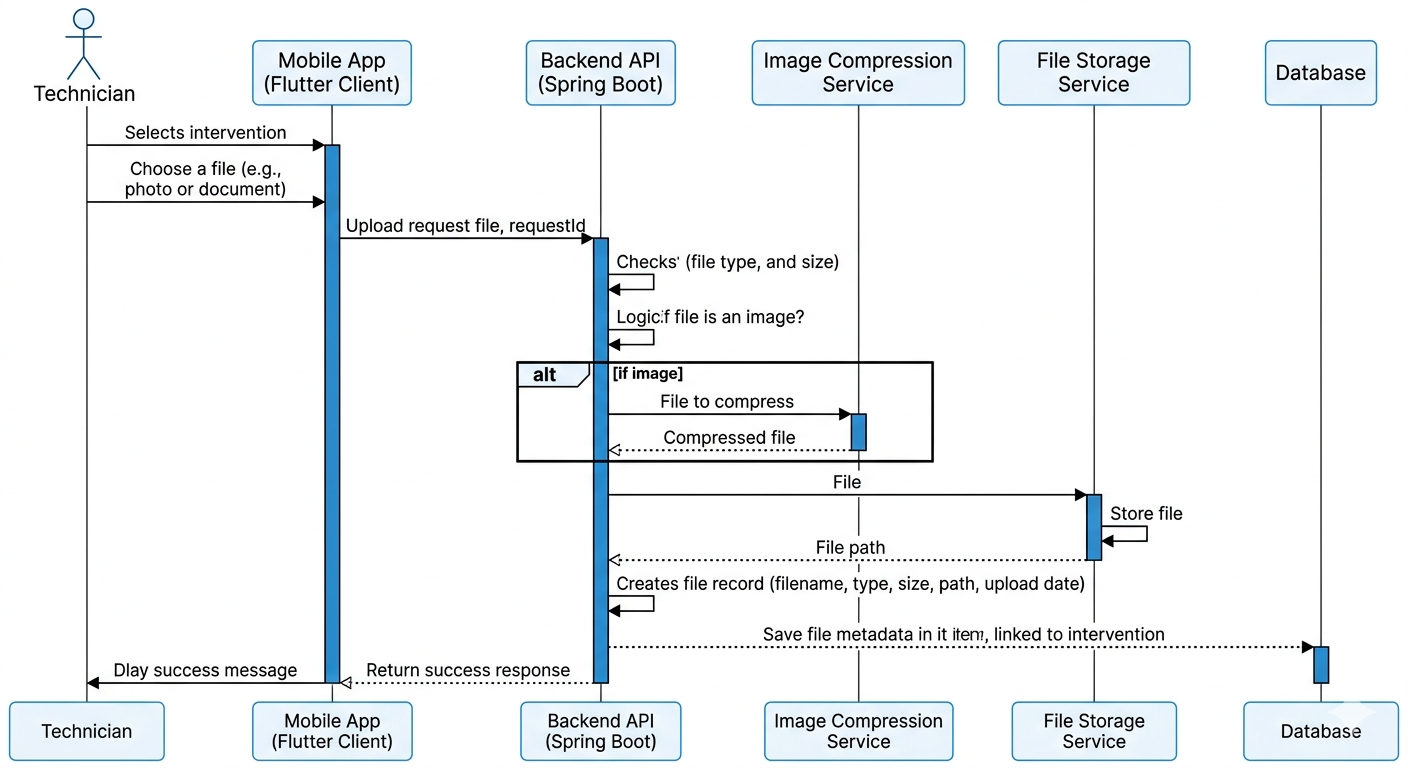
\includegraphics[width=1\textwidth]{seqFile.png} 
Sequence diagram illustrating the file upload and management process during Sprint 3.
}}
\caption{Sprint 3 File Upload and Management Sequence}
\label{fig:sprint3_sequence_file}
\end{figure}

\section{Realization}

\subsection{Backend Implementation Details}

The backend implementation in Sprint 3 focused on extending the intervention domain with file management and geolocation tracking capabilities.

\begin{itemize}
\item Secure file upload and storage with metadata persistence
\item Image compression and optimization before storage
\item File-to-intervention association management
\item Geolocation data capture and persistence linked to intervention execution
\item Access control for file retrieval and download operations
\end{itemize}

File management is handled through a dedicated service layer responsible for validating file size and type, applying compression for image files, and delegating storage to the file system or storage provider. Each uploaded file is persisted with metadata including filename, type, size, and storage path, and is linked to a specific intervention request.

Geolocation tracking is integrated into the execution workflow by associating latitude, longitude, and timestamps with each intervention. This enables traceability of technician activities and verification of intervention locations.

Primary endpoint groups delivered:

\begin{itemize}
\item \api{files}
\item \api{files/download}
\item \api{execution-details}
\end{itemize}

\subsection{Frontend Implementation}

The Angular web application was extended to support file management and evidence visualization features for supervisors and coordinators.

\begin{itemize}
\item File listing interface within intervention details view
\item Download and preview functionality for uploaded documents and images
\item Integration of evidence files into intervention tracking screens
\item Visualization of geolocation data associated with interventions
\end{itemize}

The UI enables users to access all files attached to an intervention, download them securely, and share them with external stakeholders. Location data is displayed in a structured format, allowing supervisors to verify execution locations.

\begin{figure}[H]
\centering
\fbox{\parbox{1\textwidth}{
\centering
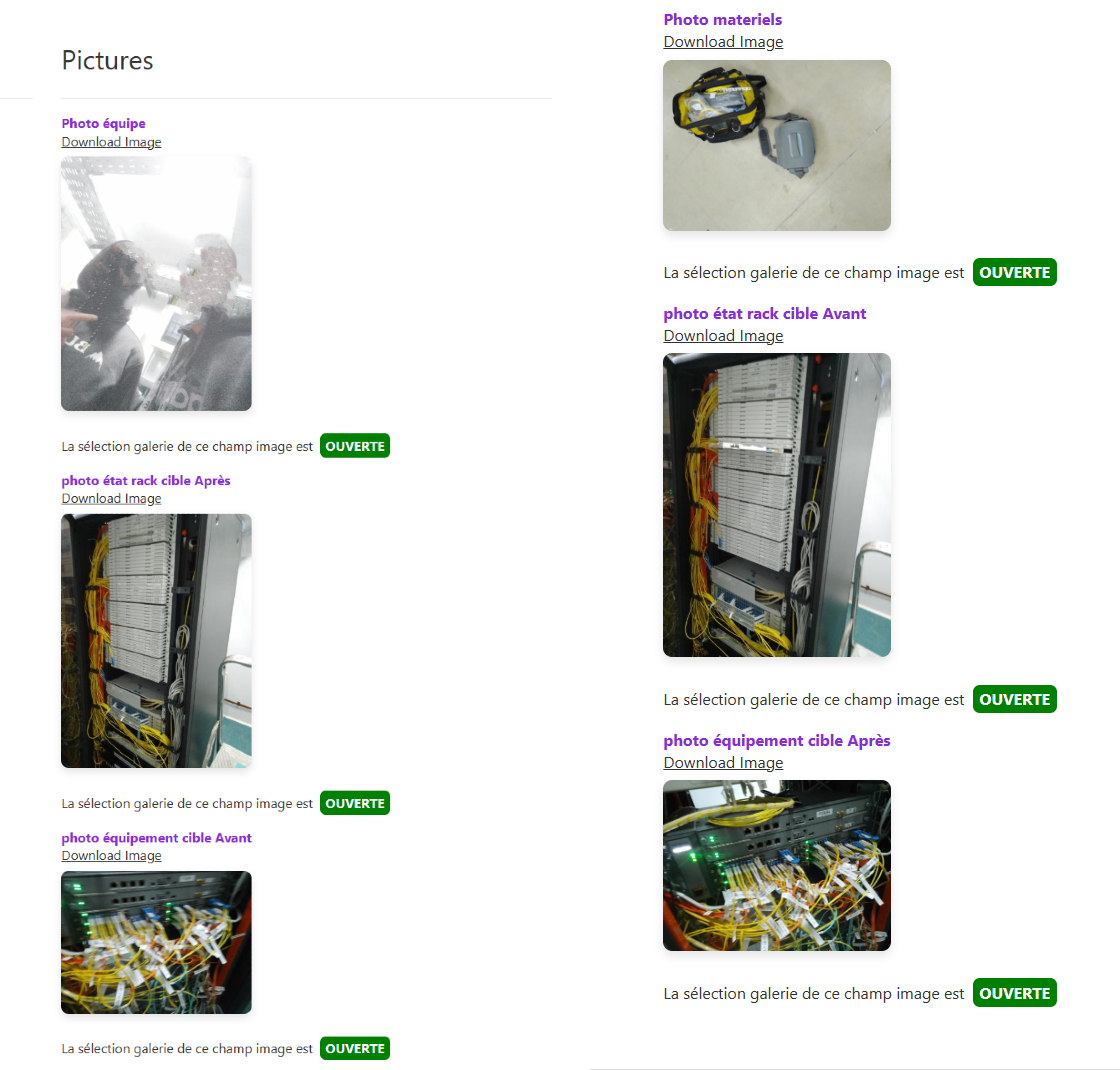
\includegraphics[width=1\textwidth]{fnial.png}
Angular UI : Intervention evidence management with file listing, download, and preview.
}}
\caption{Sprint 3 Angular UI - File Management}
\label{fig:sprint3_angular_files}
\end{figure}

\subsection{Mobile Implementation }

The Flutter mobile application was enhanced to support real-time file capture and geolocation tracking during intervention execution.

\begin{itemize}
\item Capture and upload of images and documents from device storage or camera
\item Client-side image compression before upload
\item Integration of file upload within intervention workflow
\item GPS location capture with permission handling
\item Association of location data with intervention execution
\end{itemize}

The mobile application ensures efficient data transfer by compressing images before upload and provides fallback handling for connectivity issues. Geolocation services are integrated to capture accurate position data during intervention execution.

\begin{figure}[H]
\centering
\fbox{\parbox{1\textwidth}{
\centering
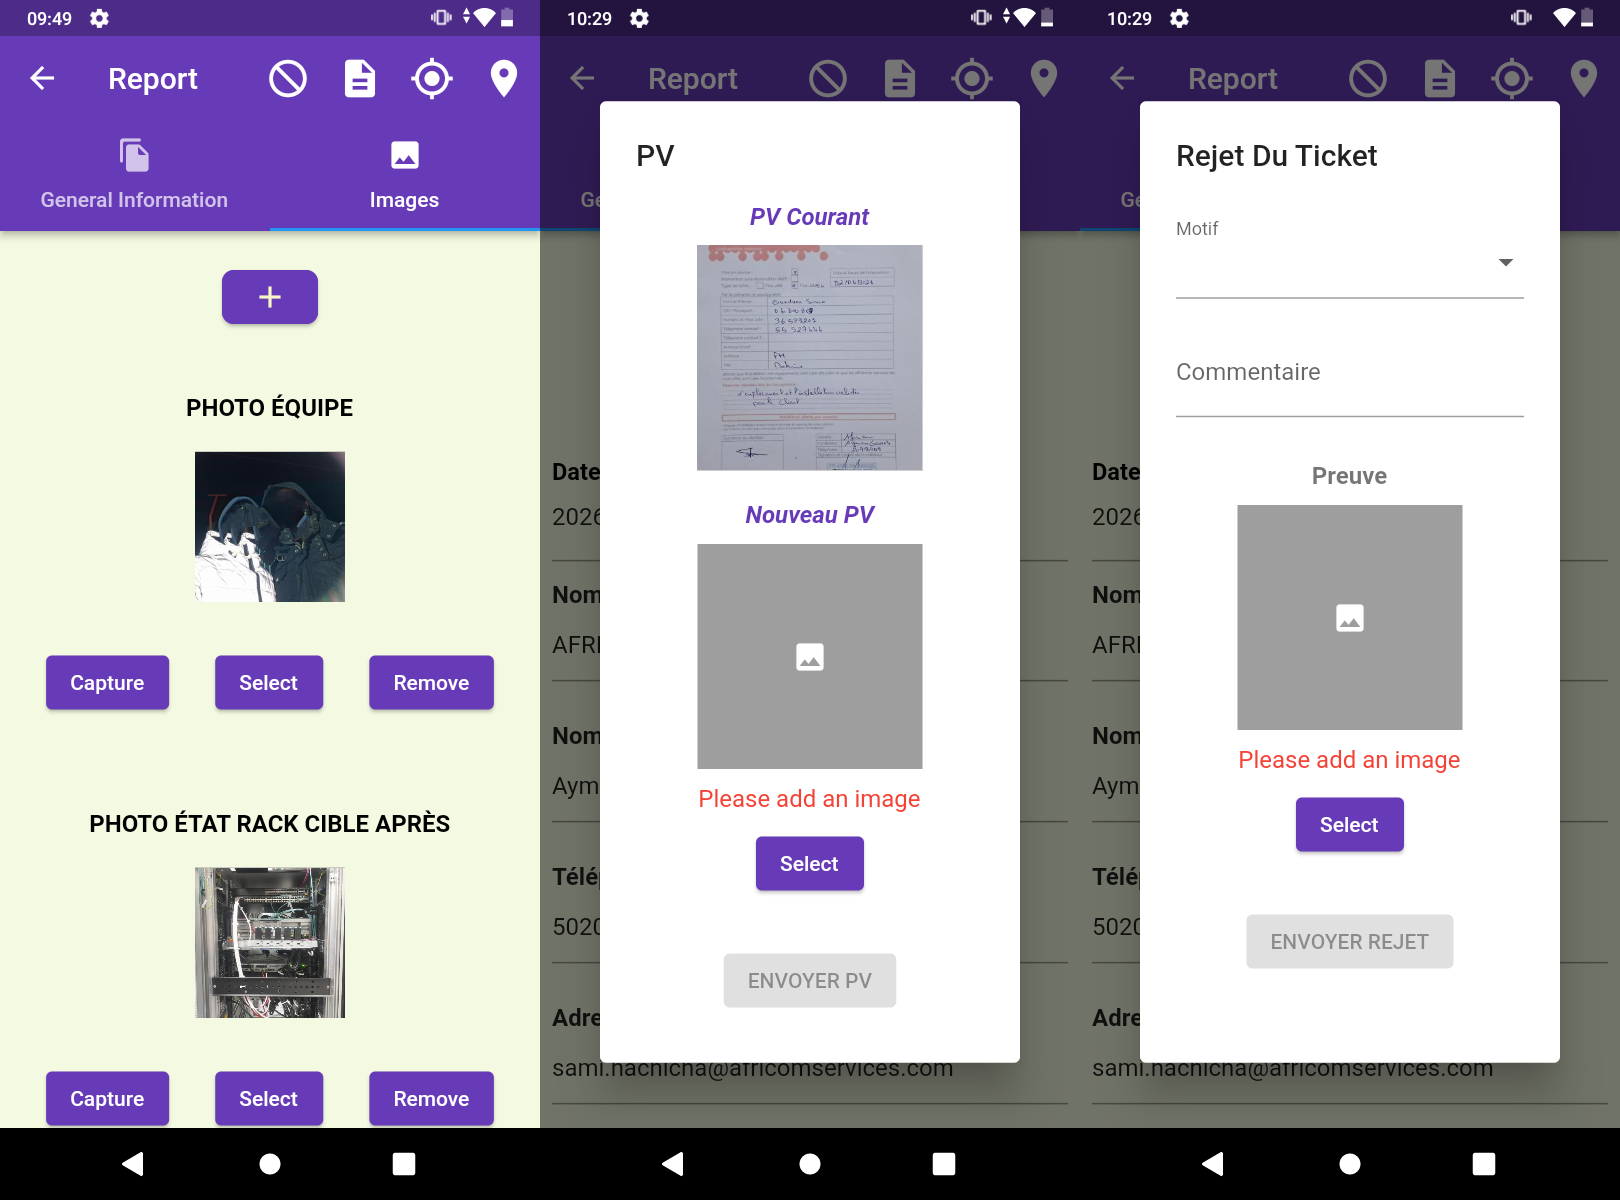
\includegraphics[width=1\textwidth]{filesFinal.png}
Flutter Mobile UI : File upload and intervention evidence capture.
}}
\caption{Sprint 3 Flutter UI - File Upload}
\label{fig:sprint3_flutter_files}
\end{figure}

\subsection{Database Design (PostgreSQL)}

Sprint 3 extended the database schema to support file storage metadata and geolocation tracking.

\begin{itemize}
\item \texttt{files} table for storing file metadata (name, type, size, path)
\item Relationship between files and intervention requests
\item \texttt{execution\_details} table for storing geolocation coordinates and timestamps
\item One-to-one association between execution details and intervention request
\end{itemize}

The database design ensures efficient storage of file references while delegating actual file content storage to the file system or external storage service. Geolocation data is structured to allow future analytics and reporting on technician movements.

\begin{figure}[H]
\centering
\fbox{\parbox{0.8\textwidth}{
\centering
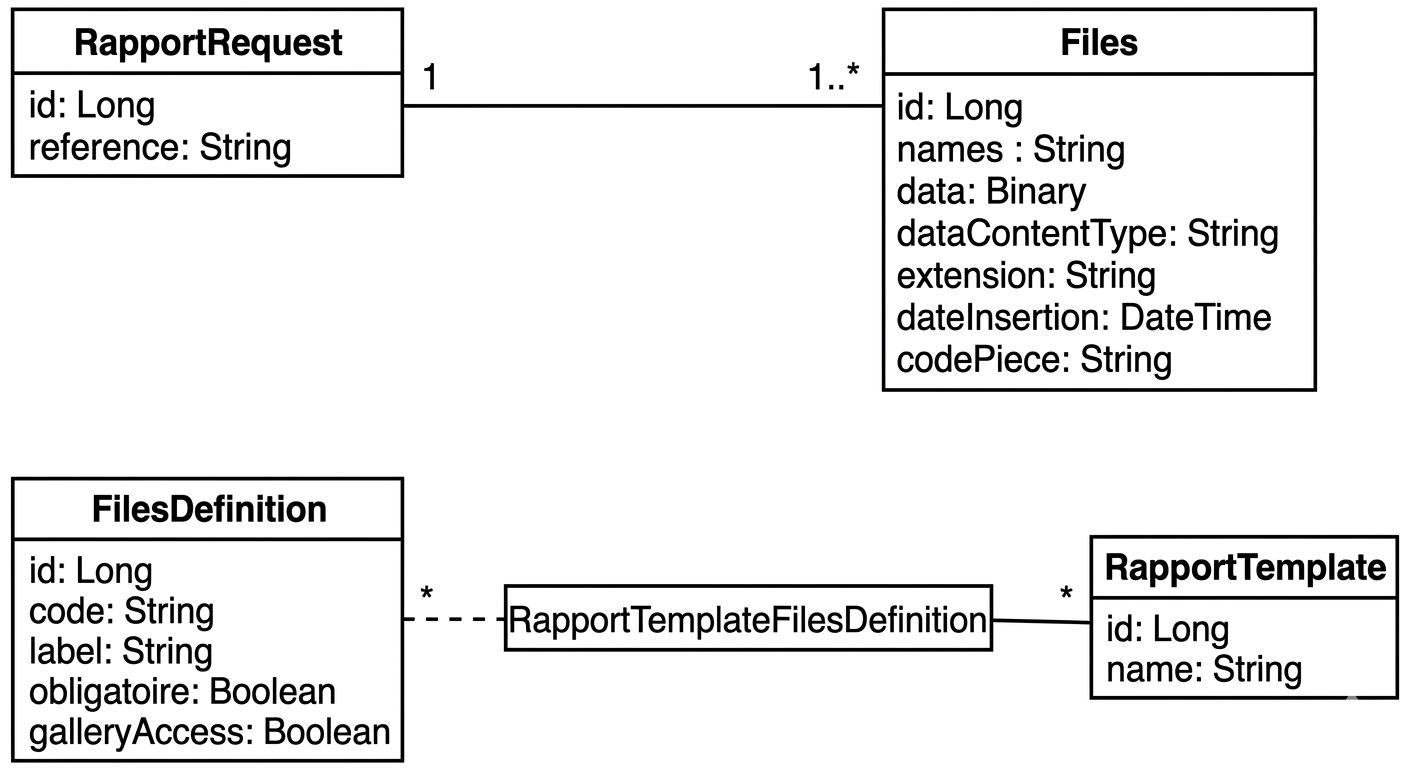
\includegraphics[width=0.8\textwidth]{dbFiles.png}
Database : File metadata
}}
\caption{Sprint 3 Database Schema}
\label{fig:sprint3_db}
\end{figure}

\subsection{API and Endpoint Summary}

\begin{table}[H]
\centering
\caption{Sprint 3 API Summary}
\label{tab:sprint3_api_summary}
\begin{tabularx}{\textwidth}{|l|l|X|}
\hline
\textbf{Method} & \textbf{Endpoint} & \textbf{Purpose} \\
\hline
POST & \api{files/upload} & Upload file and attach it to an intervention \\
\hline
GET & \api{files/{id}} & Retrieve file metadata \\
\hline
GET & \api{files/download/{id}} & Download file content securely \\
\hline
POST & \api{execution-details} & Store geolocation data for an intervention \\
\hline
GET & \api{execution-details/{requestId}} & Retrieve execution location data \\
\hline
\end{tabularx}
\end{table}

\section{Conclusion}

Sprint 3 successfully extended the system with comprehensive file management and geolocation capabilities. Technicians can now capture and upload evidence files, with automatic image compression optimizing storage while geolocation tracking provides accountability and operational insights.

Key achievements:
\begin{itemize}
\item Secure file upload and storage with access control
\item Automatic image compression and optimization
\item Mobile geolocation tracking integration
\item File download and sharing capabilities
\end{itemize}

Sprint 4 will focus on the approval workflow and status management, enabling supervisors to review and approve completed interventions.


% Chapter 7: Sprint 4
% Chapter 7: Sprint 4 - Approval Workflow & Status Management

\chapter{Sprint 4: Approval Workflow and Status Management}

\section{Introduction}

Sprint 4 implements the critical approval workflow that enables supervisors to review, validate, and approve completed interventions. This sprint introduces status tracking, audit trails, and notification mechanisms that provide transparency and control over the intervention lifecycle. The implementation ensures accountability and enables supervisors to manage quality assurance for all completed work.

The approval workflow integrates with the notification system to keep all stakeholders informed of intervention status changes, enabling efficient communication and timely decision-making throughout the organization.

\section{Sprint Preview and Objectives}

\subsection{User Stories}

\begin{enumerate}
\item \textbf{US-S4-001: Approval Workflow}
  \begin{itemize}
  \item \textbf{As a} supervisor
  \item \textbf{I want} to review and approve or reject completed interventions
  \item \textbf{So that} I ensure quality and control work delivery
  \item \textbf{Story Points:} 13
  \end{itemize}

\item \textbf{US-S4-002: Status History Tracking}
  \begin{itemize}
  \item \textbf{As a} coordinator
  \item \textbf{I want} to track status changes and reasons throughout intervention lifecycle
  \item \textbf{So that} I have complete audit trail of all modifications
  \item \textbf{Story Points:} 8
  \end{itemize}

\item \textbf{US-S4-003: Rejection with Feedback}
  \begin{itemize}
  \item \textbf{As a} supervisor
  \item \textbf{I want} to reject interventions with detailed feedback
  \item \textbf{So that} technicians understand required corrections
  \item \textbf{Story Points:} 8
  \end{itemize}

\item \textbf{US-S4-004: Status Notifications}
  \begin{itemize}
  \item \textbf{As a} system
  \item \textbf{I want} to notify stakeholders of status changes
  \item \textbf{So that} everyone is informed of intervention progress
  \item \textbf{Story Points:} 8
  \end{itemize}

\item \textbf{US-S4-005: Supervisor Dashboard}
  \begin{itemize}
  \item \textbf{As a} supervisor
  \item \textbf{I want} to view pending interventions awaiting approval
  \item \textbf{So that} I can quickly identify and process them
  \item \textbf{Story Points:} 8
  \end{itemize}
\end{enumerate}

\subsection{Sprint Goals}

\begin{enumerate}
\item \textbf{Approval Workflow:} Implement complete approval process with state transitions
\item \textbf{Status Management:} Track all status changes with audit trail
\item \textbf{Quality Assurance:} Enable supervisors to validate work and provide feedback
\item \textbf{Notifications:} Keep all stakeholders informed of status updates
\end{enumerate}

\section{Sprint Backlog}

The 45-point sprint focuses on workflow and status management:

\begin{table}[H]
\centering
\caption{Sprint 4 Backlog}
\label{tab:sprint4_backlog}
\begin{tabularx}{\textwidth}{|l|X|l|l|}
\hline
\textbf{ID} & \textbf{User Story} & \textbf{Points} & \textbf{Status} \\
\hline
S4-1 & Approval workflow & 13 & Completed \\
\hline
S4-2 & Status history tracking & 8 & Completed \\
\hline
S4-3 & Rejection with feedback & 8 & Completed \\
\hline
S4-4 & Status notifications & 8 & Completed \\
\hline
S4-5 & Supervisor dashboard & 8 & Completed \\
\hline
\textbf{Total} & & \textbf{45} & \\
\hline
\end{tabularx}
\end{table}

\section{Functional Specification}

\subsection{Intervention Status Lifecycle}

The intervention lifecycle includes the following statuses with specific transitions:

\begin{figure}[H]
\centering
\begin{tikzpicture}[
    state/.style={rectangle, draw=black, fill=lightgray, minimum width=2cm, minimum height=0.8cm},
    arrow/.style={->, thick}
  ]
  
  \node[state] (planned) at (0, 0) {PLANNED};
  \node[state] (executed) at (2.5, 0) {EXECUTED};
  \node[state] (pending) at (5, 0) {PENDING\_VALIDATION};
  \node[state] (approved) at (7.5, 0) {APPROVED};
  \node[state] (archived) at (10, 0) {ARCHIVED};
  \node[state] (rejected) at (5, -2) {REJECTED};

  \draw[arrow] (planned) -- node[above, font=\small] {Execute} (executed);
  \draw[arrow] (executed) -- node[above, font=\small] {Submit} (pending);
  \draw[arrow] (pending) -- node[above, font=\small] {Approve} (approved);
  \draw[arrow] (approved) -- node[above, font=\small] {Archive} (archived);
  \draw[arrow] (pending) -- node[left, font=\small] {Reject} (rejected);
  \draw[arrow] (rejected) -- node[below, font=\small] {Resubmit} (pending);
  
\end{tikzpicture}
\caption{Intervention Status Lifecycle}
\label{fig:sprint4_lifecycle}
\end{figure}

\section{Conception}

\subsection{Class Diagram}

\begin{figure}[H]
\centering
\begin{tikzpicture}[node distance=2cm, auto]
  \node[umlclass] (request) at (0, 2) {
    RapportRequest\\
    --------------------\\
    - id: Long\\
    - status: Status\\
    - statusHistory: Set<StatusHistory>
  };

  \node[umlclass] (status) at (3, 2) {
    StatusHistory\\
    --------------------\\
    - id: Long\\
    - previousStatus: Status\\
    - newStatus: Status\\
    - changedAt: ZonedDateTime\\
    - changedBy: User
  };

  \node[umlclass] (reject) at (3, -1) {
    Reject\\
    --------------------\\
    - id: Long\\
    - reason: String\\
    - feedback: String\\
    - rejectedAt: ZonedDateTime
  };

  \node[umlclass] (user) at (7, 2) {
    User\\
    --------------------\\
    - id: Long\\
    - login: String\\
    - role: Role
  };

  \draw[->] (request) -- (status) node[midway, above] {has};
  \draw[->] (status) -- (user) node[midway, above] {trackedBy};
  \draw[->] (request) -- (reject) node[midway, right] {may have};

\end{tikzpicture}
\caption{Sprint 4 Class Diagram - Approval Workflow}
\label{fig:sprint4_class}
\end{figure}

\section{Realization}

\subsection{Backend Implementation}

\textbf{Status Enumeration:}
\begin{lstlisting}
public enum RapportStatus {
    PLANNED("Planifie"),
    EXECUTED("Excute"),
    PENDING_VALIDATION("En attente de validation"),
    APPROVED("Approuve"),
    REJECTED("Rejete"),
    ARCHIVED("Archive");

    private final String label;

    RapportStatus(String label) {
        this.label = label;
    }
}
\end{lstlisting}

\textbf{StatusHistory Entity:}
\begin{lstlisting}
@Entity
@Table(name = "status_history")
public class StatusHistory extends AbstractAuditingEntity {

    @Id
    @GeneratedValue(strategy = GenerationType.SEQUENCE)
    private Long id;

    @Enumerated(EnumType.STRING)
    private RapportStatus previousStatus;

    @Enumerated(EnumType.STRING)
    private RapportStatus newStatus;

    @Column(name = "changed_at")
    private ZonedDateTime changedAt;

    @ManyToOne
    private User changedBy;

    @ManyToOne
    private RapportRequest rapportRequest;
}
\end{lstlisting}

\textbf{Rejection Entity:}
\begin{lstlisting}
@Entity
@Table(name = "rejection")
public class Rejection {

    @Id
    @GeneratedValue(strategy = GenerationType.SEQUENCE)
    private Long id;

    @Column(name = "reason")
    private String reason;

    @Column(name = "feedback", columnDefinition = "TEXT")
    private String feedback;

    @Column(name = "rejected_at")
    private ZonedDateTime rejectedAt;

    @ManyToOne
    private User rejectedBy;

    @OneToOne
    private RapportRequest rapportRequest;
}
\end{lstlisting}

\textbf{Approval Service:}
\begin{lstlisting}
@Service
@Transactional
public class ApprovalService {

    private final RapportRequestRepository requestRepository;
    private final StatusHistoryRepository historyRepository;
    private final RejectionRepository rejectionRepository;
    private final NotificationService notificationService;
    private final CurrentUserService currentUser;

    public RapportRequestDTO approveIntervention(Long requestId) {
        RapportRequest request = requestRepository.findById(requestId)
            .orElseThrow();

        if (request.getStatus() != RapportStatus.PENDING_VALIDATION) {
            throw new InvalidStatusTransitionException();
        }

        // Record status change
        StatusHistory history = new StatusHistory();
        history.setPreviousStatus(request.getStatus());
        history.setNewStatus(RapportStatus.APPROVED);
        history.setChangedAt(ZonedDateTime.now());
        history.setChangedBy(currentUser.getCurrentUser());
        history.setRapportRequest(request);
        historyRepository.save(history);

        // Update request
        request.setStatus(RapportStatus.APPROVED);
        request = requestRepository.save(request);

        // Send notification
        notificationService.notifyApproval(request);

        return mapper.toDto(request);
    }

    public RapportRequestDTO rejectIntervention(
        Long requestId,
        String reason,
        String feedback) {

        RapportRequest request = requestRepository.findById(requestId)
            .orElseThrow();

        if (request.getStatus() != RapportStatus.PENDING_VALIDATION) {
            throw new InvalidStatusTransitionException();
        }

        // Create rejection record
        Rejection rejection = new Rejection();
        rejection.setReason(reason);
        rejection.setFeedback(feedback);
        rejection.setRejectedAt(ZonedDateTime.now());
        rejection.setRejectedBy(currentUser.getCurrentUser());
        rejection.setRapportRequest(request);
        rejectionRepository.save(rejection);

        // Update status
        StatusHistory history = new StatusHistory();
        history.setPreviousStatus(request.getStatus());
        history.setNewStatus(RapportStatus.REJECTED);
        history.setChangedAt(ZonedDateTime.now());
        history.setChangedBy(currentUser.getCurrentUser());
        history.setRapportRequest(request);
        historyRepository.save(history);

        request.setStatus(RapportStatus.REJECTED);
        request = requestRepository.save(request);

        // Notify technician of rejection
        notificationService.notifyRejection(request, feedback);

        return mapper.toDto(request);
    }
}
\end{lstlisting}

\textbf{REST Controller:}
\begin{lstlisting}
@RestController
@RequestMapping("/api/rapport-requests")
public class ApprovalController {

    private final ApprovalService approvalService;

    @PostMapping("/{id}/approve")
    @PreAuthorize("hasRole('SUPERVISOR')")
    public ResponseEntity<RapportRequestDTO> approve(@PathVariable Long id) {
        return ResponseEntity.ok(approvalService.approveIntervention(id));
    }

    @PostMapping("/{id}/reject")
    @PreAuthorize("hasRole('SUPERVISOR')")
    public ResponseEntity<RapportRequestDTO> reject(
        @PathVariable Long id,
        @RequestBody RejectionDTO rejectionDTO) {

        return ResponseEntity.ok(approvalService.rejectIntervention(
            id,
            rejectionDTO.getReason(),
            rejectionDTO.getFeedback()
        ));
    }

    @GetMapping("/pending")
    @PreAuthorize("hasRole('SUPERVISOR')")
    public ResponseEntity<Page<RapportRequestDTO>> getPendingRequests(
        @PageableDefault(size = 20) Pageable pageable) {

        Page<RapportRequest> pending = requestRepository.findByStatus(
            RapportStatus.PENDING_VALIDATION,
            pageable);

        return ResponseEntity.ok(pending.map(mapper::toDto));
    }

    @GetMapping("/{id}/history")
    public ResponseEntity<List<StatusHistoryDTO>> getStatusHistory(@PathVariable Long id) {
        List<StatusHistory> history = historyRepository.findByRapportRequestId(id);
        return ResponseEntity.ok(history.stream()
            .map(mapper::toDto)
            .collect(Collectors.toList()));
    }
}
\end{lstlisting}

\subsection{Frontend Implementation}

\textbf{Approval Component:}
\begin{lstlisting}
@Component({
  selector: 'app-approval',
  templateUrl: './approval.component.html',
  styleUrls: ['./approval.component.css']
})
export class ApprovalComponent implements OnInit {
  pendingInterventions: RapportRequest[] = [];
  selectedIntervention: RapportRequest | null = null;
  rejectionForm: FormGroup;
  isLoading = false;

  constructor(
    private rapportService: RapportRequestService,
    private formBuilder: FormBuilder,
    private notificationService: NotificationService
  ) {
    this.rejectionForm = this.formBuilder.group({
      reason: ['', Validators.required],
      feedback: ['', Validators.required]
    });
  }

  ngOnInit(): void {
    this.loadPendingInterventions();
  }

  loadPendingInterventions(): void {
    this.isLoading = true;
    this.rapportService.getPendingApprovals()
      .subscribe({
        next: (data) => {
          this.pendingInterventions = data;
          this.isLoading = false;
        },
        error: () => this.isLoading = false
      });
  }

  approve(intervention: RapportRequest): void {
    if (!confirm('Are you sure you want to approve this intervention?')) {
      return;
    }

    this.rapportService.approveIntervention(intervention.id)
      .subscribe({
        next: () => {
          this.notificationService.showSuccess(
            'Intervention approved successfully');
          this.loadPendingInterventions();
        },
        error: (error) => {
          this.notificationService.showError(
            'Failed to approve intervention');
        }
      });
  }

  reject(intervention: RapportRequest): void {
    if (this.rejectionForm.invalid) {
      return;
    }

    this.rapportService.rejectIntervention(
      intervention.id,
      this.rejectionForm.value)
      .subscribe({
        next: () => {
          this.notificationService.showSuccess(
            'Intervention rejected');
          this.rejectionForm.reset();
          this.loadPendingInterventions();
        },
        error: () => {
          this.notificationService.showError(
            'Failed to reject intervention');
        }
      });
  }

  viewHistory(intervention: RapportRequest): void {
    this.rapportService.getStatusHistory(intervention.id)
      .subscribe((history) => {
        // Display status history dialog
      });
  }
}
\end{lstlisting}

\section{Tests and Validation}

\subsubsection{Approval Workflow Tests}

\begin{lstlisting}
@SpringBootTest
class ApprovalServiceTest {

    @Autowired
    private ApprovalService approvalService;

    @MockBean
    private NotificationService notificationService;

    @Test
    void approveIntervention() {
        RapportRequest request = createPendingIntervention();

        RapportRequestDTO result = approvalService
            .approveIntervention(request.getId());

        assertThat(result.getStatus()).isEqualTo(RapportStatus.APPROVED);
        verify(notificationService).notifyApproval(any());
    }

    @Test
    void rejectIntervention() {
        RapportRequest request = createPendingIntervention();

        RapportRequestDTO result = approvalService.rejectIntervention(
            request.getId(),
            "Missing information",
            "Please provide additional photos");

        assertThat(result.getStatus()).isEqualTo(RapportStatus.REJECTED);
        verify(notificationService).notifyRejection(any(), anyString());
    }

    @Test
    void validateStatusTransitions() {
        RapportRequest request = createArchivedIntervention();

        assertThatThrownBy(() -> 
            approvalService.approveIntervention(request.getId()))
            .isInstanceOf(InvalidStatusTransitionException.class);
    }
}
\end{lstlisting}

\section{Conclusion}

Sprint 4 successfully implemented the approval workflow and comprehensive status management system. Supervisors now have complete visibility and control over the intervention lifecycle, with detailed audit trails tracking all status changes. The rejection workflow enables constructive feedback and continuous improvement, while notifications ensure stakeholders remain informed of all changes.

Key achievements:
\begin{itemize}
\item Complete approval workflow with state transitions
\item Status history tracking for full audit trail
\item Rejection with detailed feedback mechanism
\item Real-time notifications for status changes
\item Supervisor dashboard for pending reviews
\end{itemize}

Sprint 5 will focus on advanced reporting capabilities and system optimization, enabling comprehensive analysis of intervention data and operational metrics.


% Chapter 8: Sprint 5
% Chapter 8: Sprint 5 - Excel Report Generation & System Optimization

\chapter{Sprint 5: Excel Report Generation and System Optimization}

\section{Introduction}

Sprint 5, the final development sprint, implements advanced reporting capabilities and system optimization. This sprint delivers comprehensive Excel report generation enabling stakeholders to analyze intervention data, create organizational archives, and perform metrics analysis. System optimization ensures scalability, performance, and reliability in production environments.

The sprint focuses on business analytics and operational intelligence, providing management with tools to monitor operations, identify trends, and make data-driven decisions. Performance optimization ensures the system can handle growing data volumes and concurrent user load effectively.

\section{Sprint Preview and Objectives}

\subsection{User Stories}

\begin{enumerate}
\item \textbf{US-S5-001: Excel Report Generation}
  \begin{itemize}
  \item \textbf{As a} coordinator
  \item \textbf{I want} to generate comprehensive Excel reports from intervention data
  \item \textbf{So that} I can analyze and share intervention metrics
  \item \textbf{Story Points:} 13
  \end{itemize}

\item \textbf{US-S5-002: Dynamic Report Templates}
  \begin{itemize}
  \item \textbf{As a} manager
  \item \textbf{I want} to configure custom Excel templates for reports
  \item \textbf{So that} reports match organizational standards
  \item \textbf{Story Points:} 8
  \end{itemize}

\item \textbf{US-S5-003: Archive Management}
  \begin{itemize}
  \item \textbf{As a} system
  \item \textbf{I want} to automatically archive old interventions
  \item \textbf{So that} database remains performant
  \item \textbf{Story Points:} 8
  \end{itemize}

\item \textbf{US-S5-004: Performance Optimization}
  \begin{itemize}
  \item \textbf{As a} system
  \item \textbf{I want} to optimize queries and caching
  \item \textbf{So that} system handles large datasets efficiently
  \item \textbf{Story Points:} 8
  \end{itemize}

\item \textbf{US-S5-005: System Monitoring}
  \begin{itemize}
  \item \textbf{As a} administrator
  \item \textbf{I want} to monitor system health and metrics
  \item \textbf{So that} I can identify and resolve issues proactively
  \item \textbf{Story Points:} 8
  \end{itemize}
\end{enumerate}

\subsection{Sprint Goals}

\begin{enumerate}
\item \textbf{Reporting:} Implement comprehensive Excel report generation
\item \textbf{Configuration:} Enable customizable report templates
\item \textbf{Archive:} Implement intelligent data archival strategy
\item \textbf{Performance:} Optimize system for scalability
\item \textbf{Monitoring:} Provide system health visibility
\end{enumerate}

\section{Sprint Backlog}

The 45-point sprint focuses on advanced features and optimization:

\begin{table}[H]
\centering
\caption{Sprint 5 Backlog}
\label{tab:sprint5_backlog}
\begin{tabularx}{\textwidth}{|l|X|l|l|}
\hline
\textbf{ID} & \textbf{User Story} & \textbf{Points} & \textbf{Status} \\
\hline
S5-1 & Excel report generation & 13 & Completed \\
\hline
S5-2 & Dynamic report templates & 8 & Completed \\
\hline
S5-3 & Archive management & 8 & Completed \\
\hline
S5-4 & Performance optimization & 8 & Completed \\
\hline
S5-5 & System monitoring & 8 & Completed \\
\hline
\textbf{Total} & & \textbf{45} & \\
\hline
\end{tabularx}
\end{table}

\section{Functional Specification}

\subsection{Report Generation Process}

The Excel report generation process involves:

\begin{enumerate}
\item \textbf{Data Collection:} Query interventions based on filters
\item \textbf{Template Loading:} Retrieve active report template configuration
\item \textbf{Dynamic Population:} Insert data into Excel using Apache POI
\item \textbf{Calculation:} Compute metrics and aggregations
\item \textbf{Styling:} Apply formatting and themes
\item \textbf{Export:} Generate and download Excel file
\end{enumerate}

\subsection{Report Types}

\begin{itemize}
\item \textbf{Daily Summary:} Interventions completed by day with metrics
\item \textbf{Technician Report:} Performance by technician
\item \textbf{Regional Report:} Geographic analysis of work
\item \textbf{Custom Report:} User-defined filters and metrics
\end{itemize}

\section{Conception}

\subsection{Class Diagram}

\begin{figure}[H]
\centering
\fbox{\parbox{1\textwidth}{
\centering
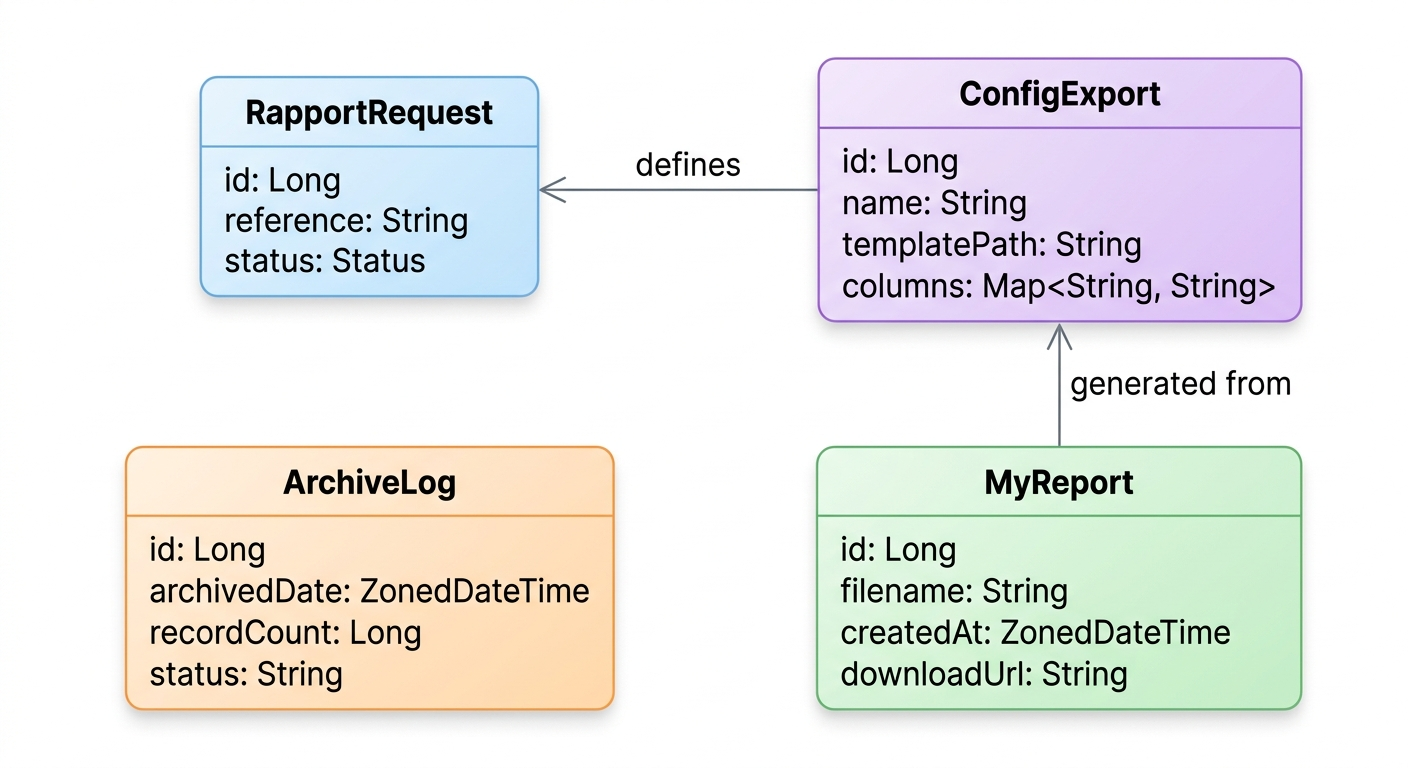
\includegraphics[width=1\textwidth]{class.png}
Class diagram illustrating the Report Manager system
}}
\caption{Sprint 5 Class Diagram}
\label{fig:sprint5_class}
\end{figure}

\section{Realization}

\subsection{Architecture Overview}

Sprint 5 realization focused on two main goals:

\begin{itemize}
\item \textbf{Advanced Reporting:} Enable dynamic Excel report generation based on configurable templates and user-defined filters.
\item \textbf{System Optimization:} Ensure scalability, query efficiency, caching, and automated archival for high-volume intervention data.
\end{itemize}

% The system leverages existing intervention and template domains while adding new services and configurations for reporting and optimization.

\subsection{Backend Implementation Logic}

% Backend services were designed to handle configurable, scalable, and reusable reporting operations:

\begin{itemize}
\item \textbf{ConfigExport Service:} Manages report templates with dynamic column mapping and template activation.
\item \textbf{ExcelReportService:} 
  \begin{itemize}
    \item Queries intervention data based on dynamic filters.
    \item Populates Excel reports using the configured template mapping.
    \item Computes metrics and aggregates without hard-coded field displays.
    \item Handles file creation, storage, and download preparation.
  \end{itemize}
\item \textbf{ArchiveService:} 
  \begin{itemize}
    \item Implements automatic archival of old interventions.
    \item Integrates with external storage solutions for cold data.
    \item A scheduled Maven-based cron job runs every day at 3:00 AM according to project specifications.
    \item It retrieves and processes images of tickets exceeding the days to archive threshold in the \texttt{rapport\_template} table.
    \item It stores archived images in a backup machine, ensuring consistent and reliable data preservation.
  \end{itemize}
\item \textbf{REST Controllers:} Expose endpoints for:
  \begin{itemize}
    \item Dynamic report generation.
    \item Configurable template CRUD operations.
    \item Filtered intervention retrieval for reporting.
  \end{itemize}
\end{itemize}

\subsection{Performance and Optimization Logic}

\begin{itemize}
\item \textbf{Query Optimization:} JPA specifications and fetch strategies avoid N+1 queries, and support large datasets efficiently.
\item \textbf{Caching:} Frequently accessed data (e.g., report templates, intervention summaries) is cached for faster retrieval.
\item \textbf{Archival Scheduling:} Automated cron jobs archive old interventions and maintain system performance.
\item \textbf{Monitoring Integration:} Tracks key metrics such as database query performance, cache hit rates, memory usage, and request statistics.
\end{itemize}

\subsection{Frontend and Integration Logic}

\begin{itemize}
\item Dynamic Rendering of report generation options based on selected templates.
\item Users select filters and templates without hard-coded column mapping.
\item Report download is handled as a fileStream allowing seamless interaction with large datasets.
\item Archival operations are invisible to users but logged for audit purposes.
\end{itemize}

\begin{figure}[H]
\centering
\fbox{\parbox{1\textwidth}{
\centering
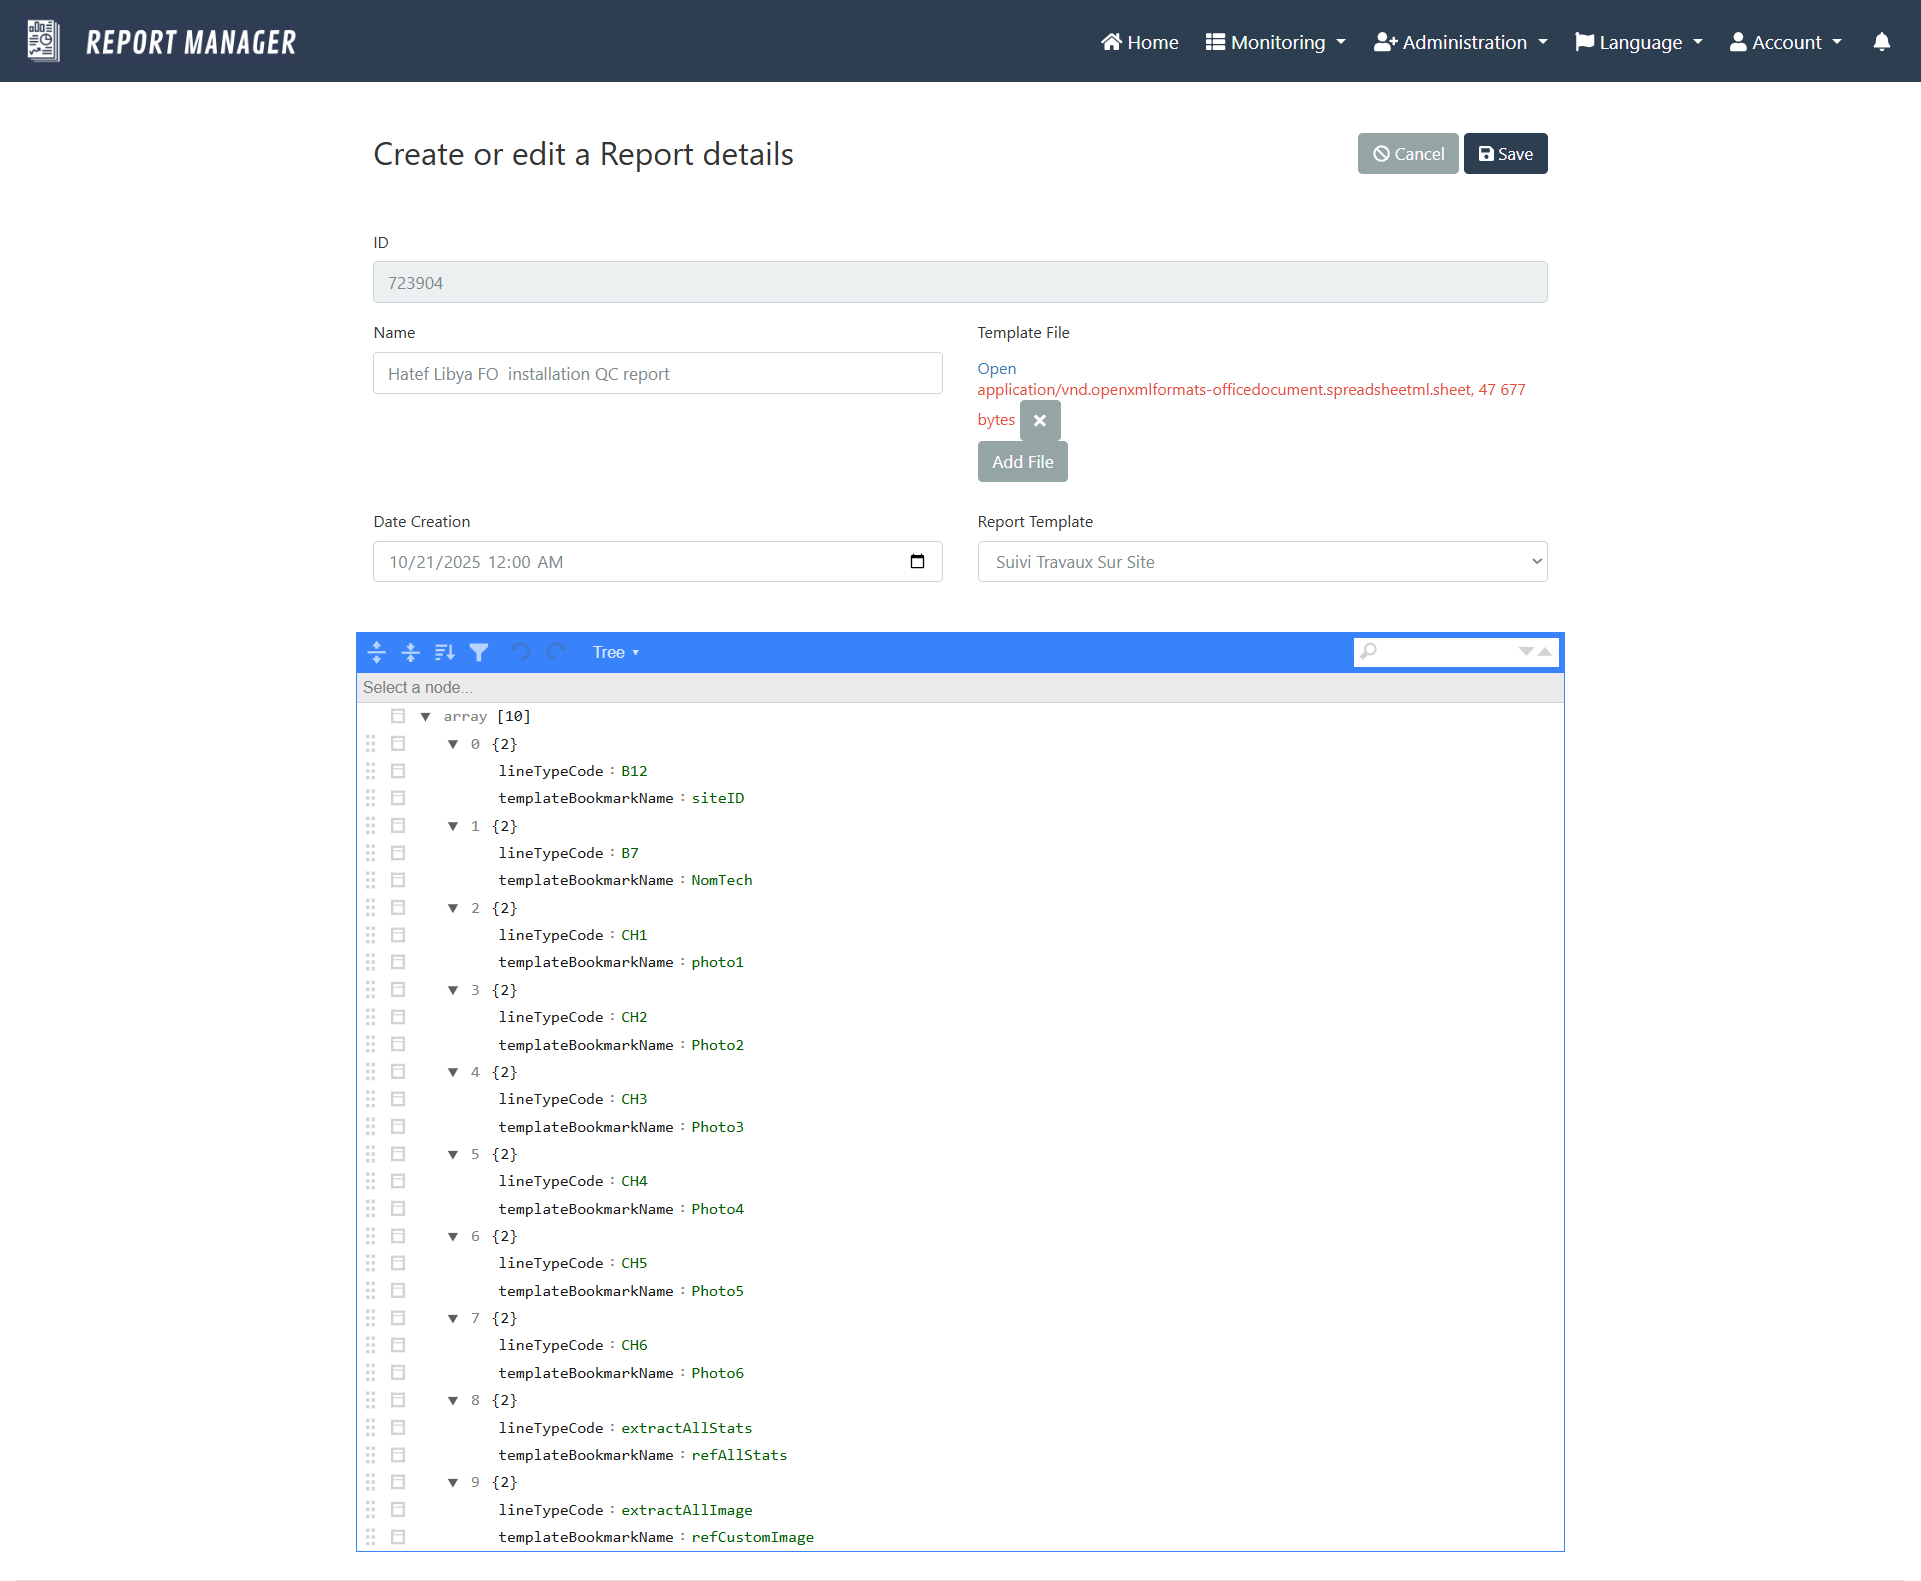
\includegraphics[width=1\textwidth]{outputDef.png}
Example of a configurable Excel report template with dynamic column mapping
}}
\caption{Sprint 5 Output Definition}
\label{fig:sprint5_output}
\end{figure}

\begin{figure}[H]
\centering
\fbox{\parbox{1\textwidth}{
\centering
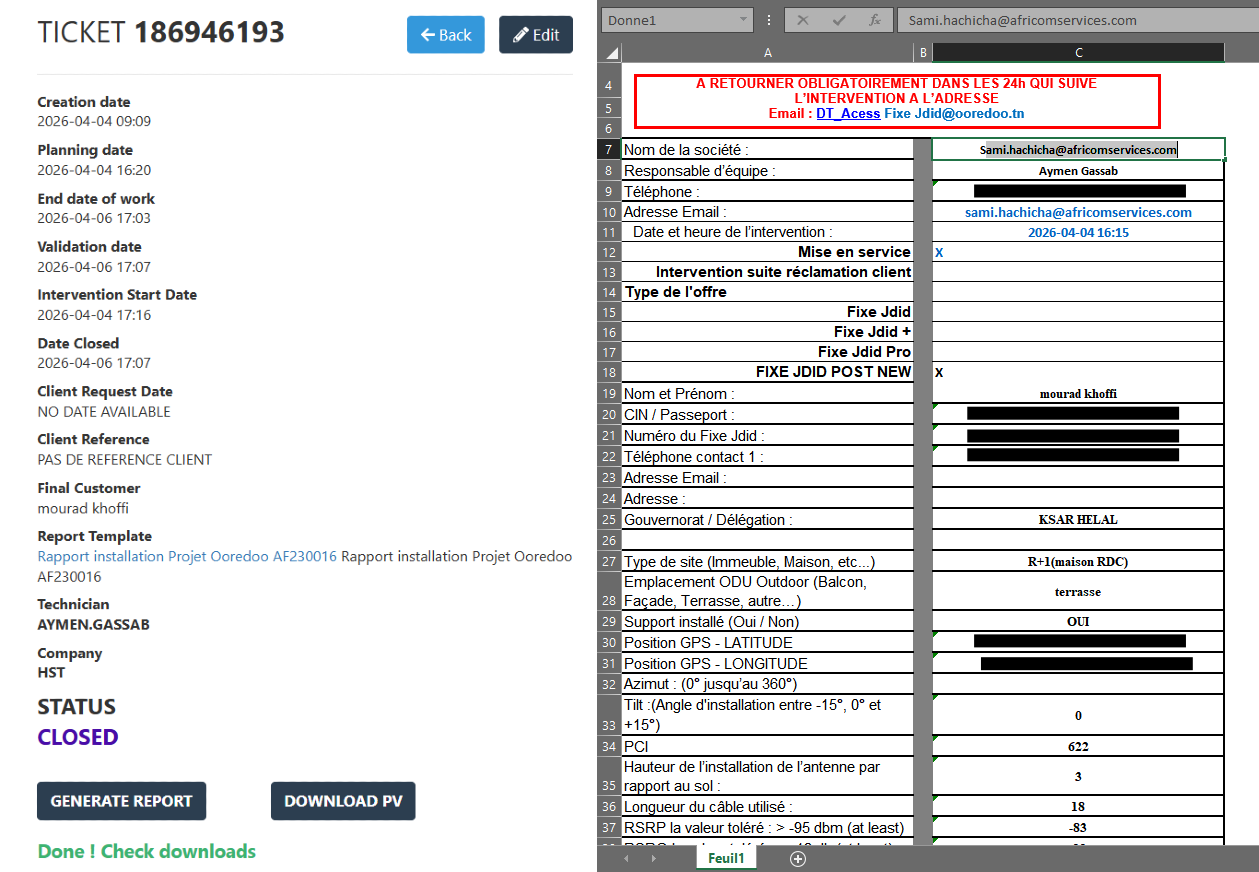
\includegraphics[width=1\textwidth]{gen.png}
Example of a dynamically generated Excel report based on intervention data
}}
\caption{Sprint 5 Generated Report}
\label{fig:sprint5_generated}
\end{figure}


\begin{figure}[H]
\centering
\fbox{\parbox{1\textwidth}{
\centering
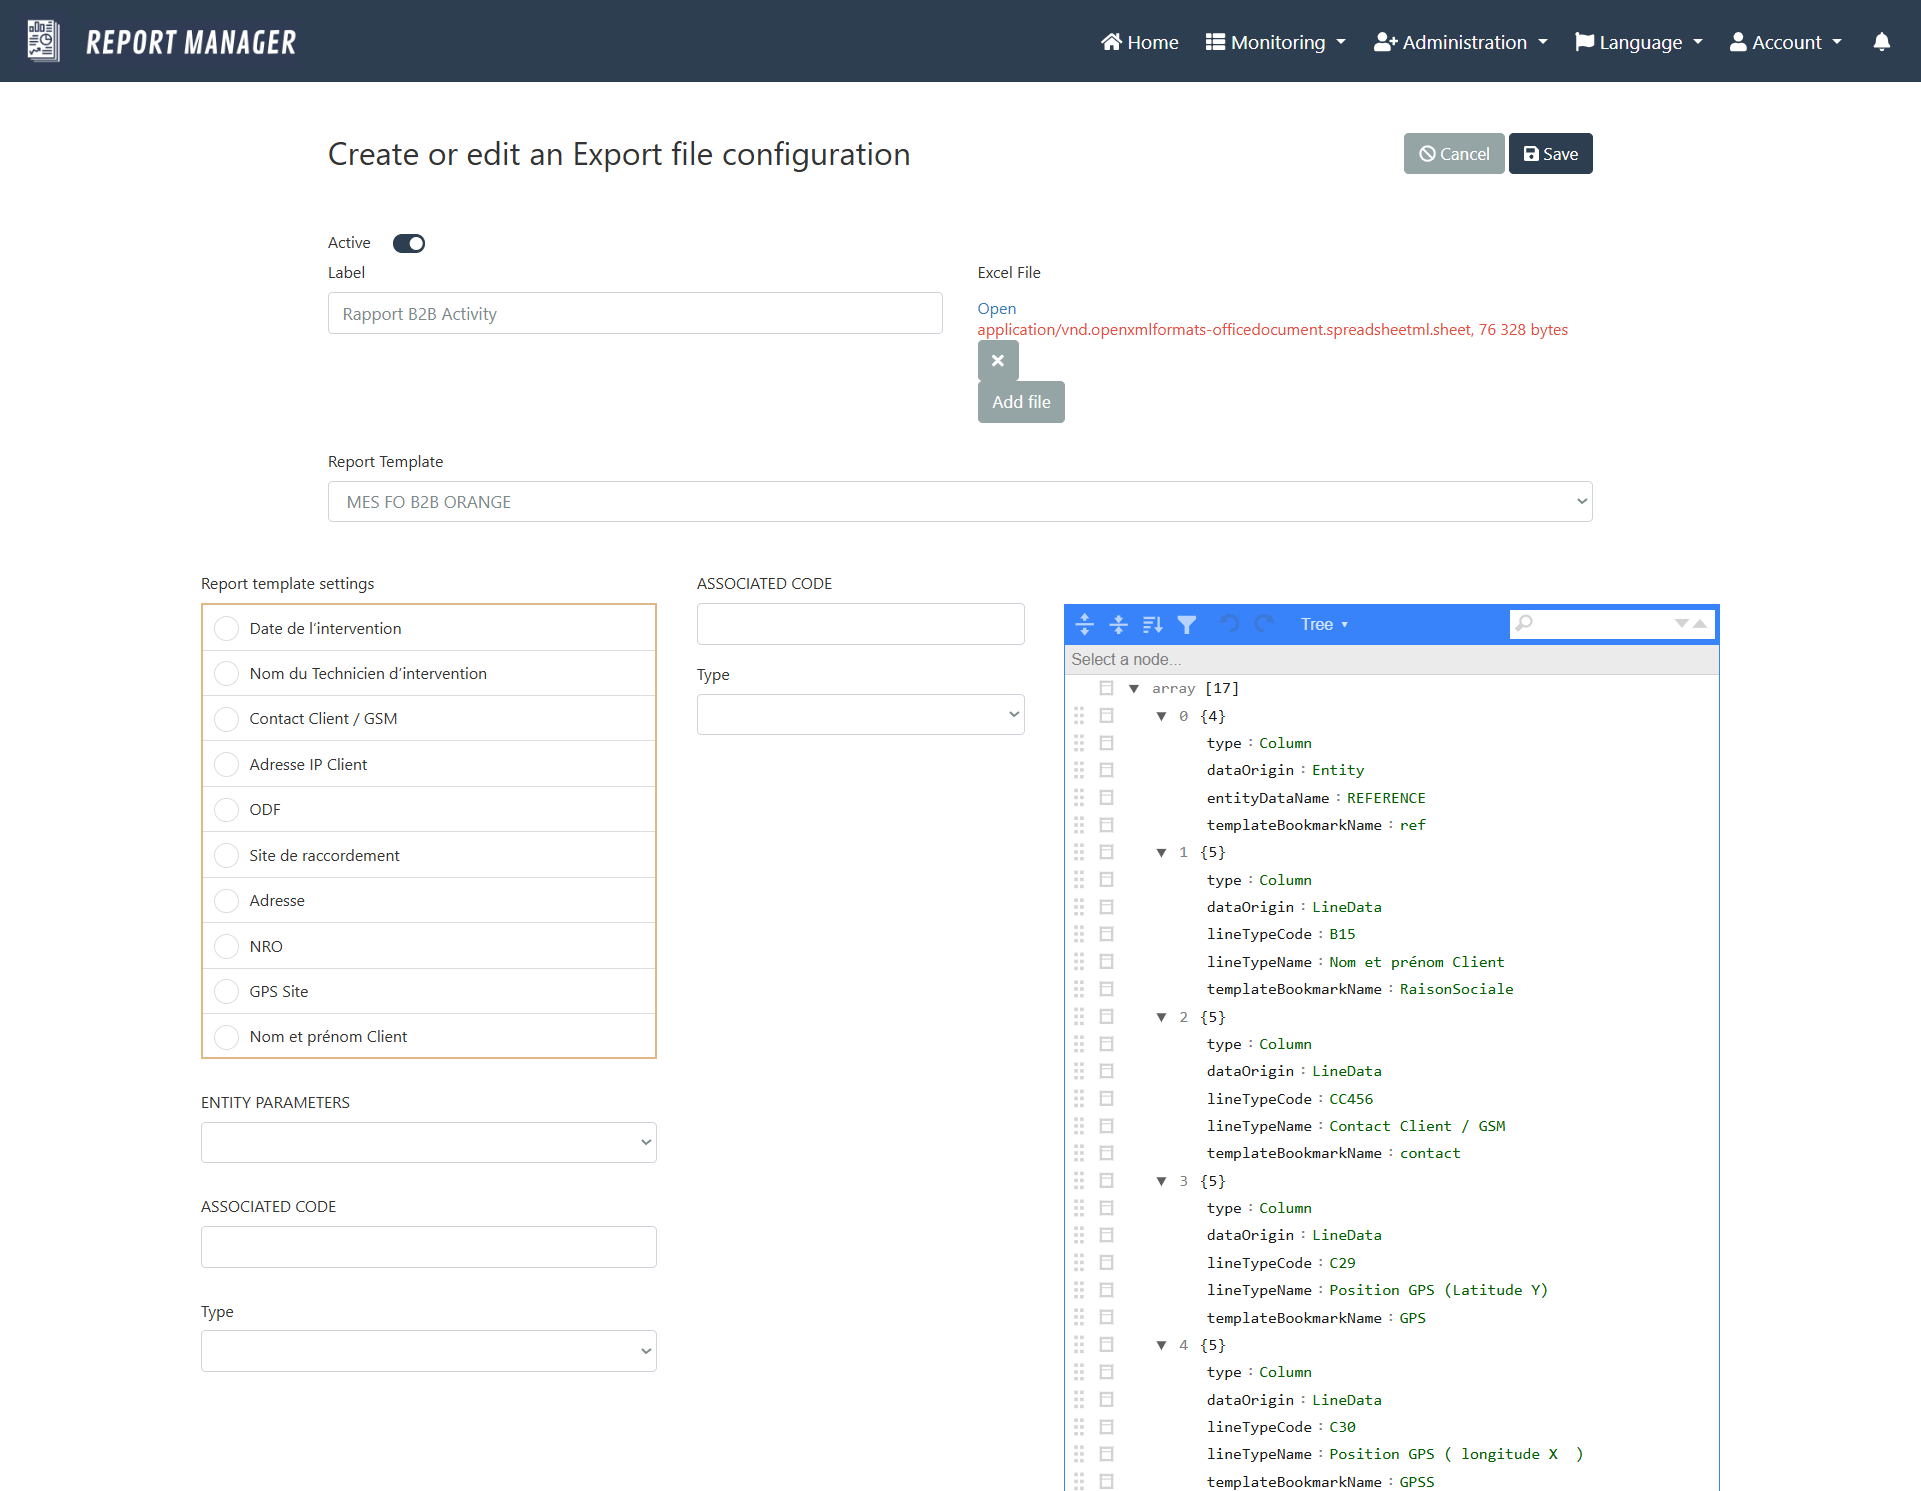
\includegraphics[width=1\textwidth]{conf1.png}
Example of a configurable Excel activity report template with dynamic column mapping
}}
\caption{Sprint 5 Configurable Template}
\label{fig:sprint5_configurable}
\end{figure}


\begin{figure}[H]
\centering
\fbox{\parbox{1\textwidth}{
\centering
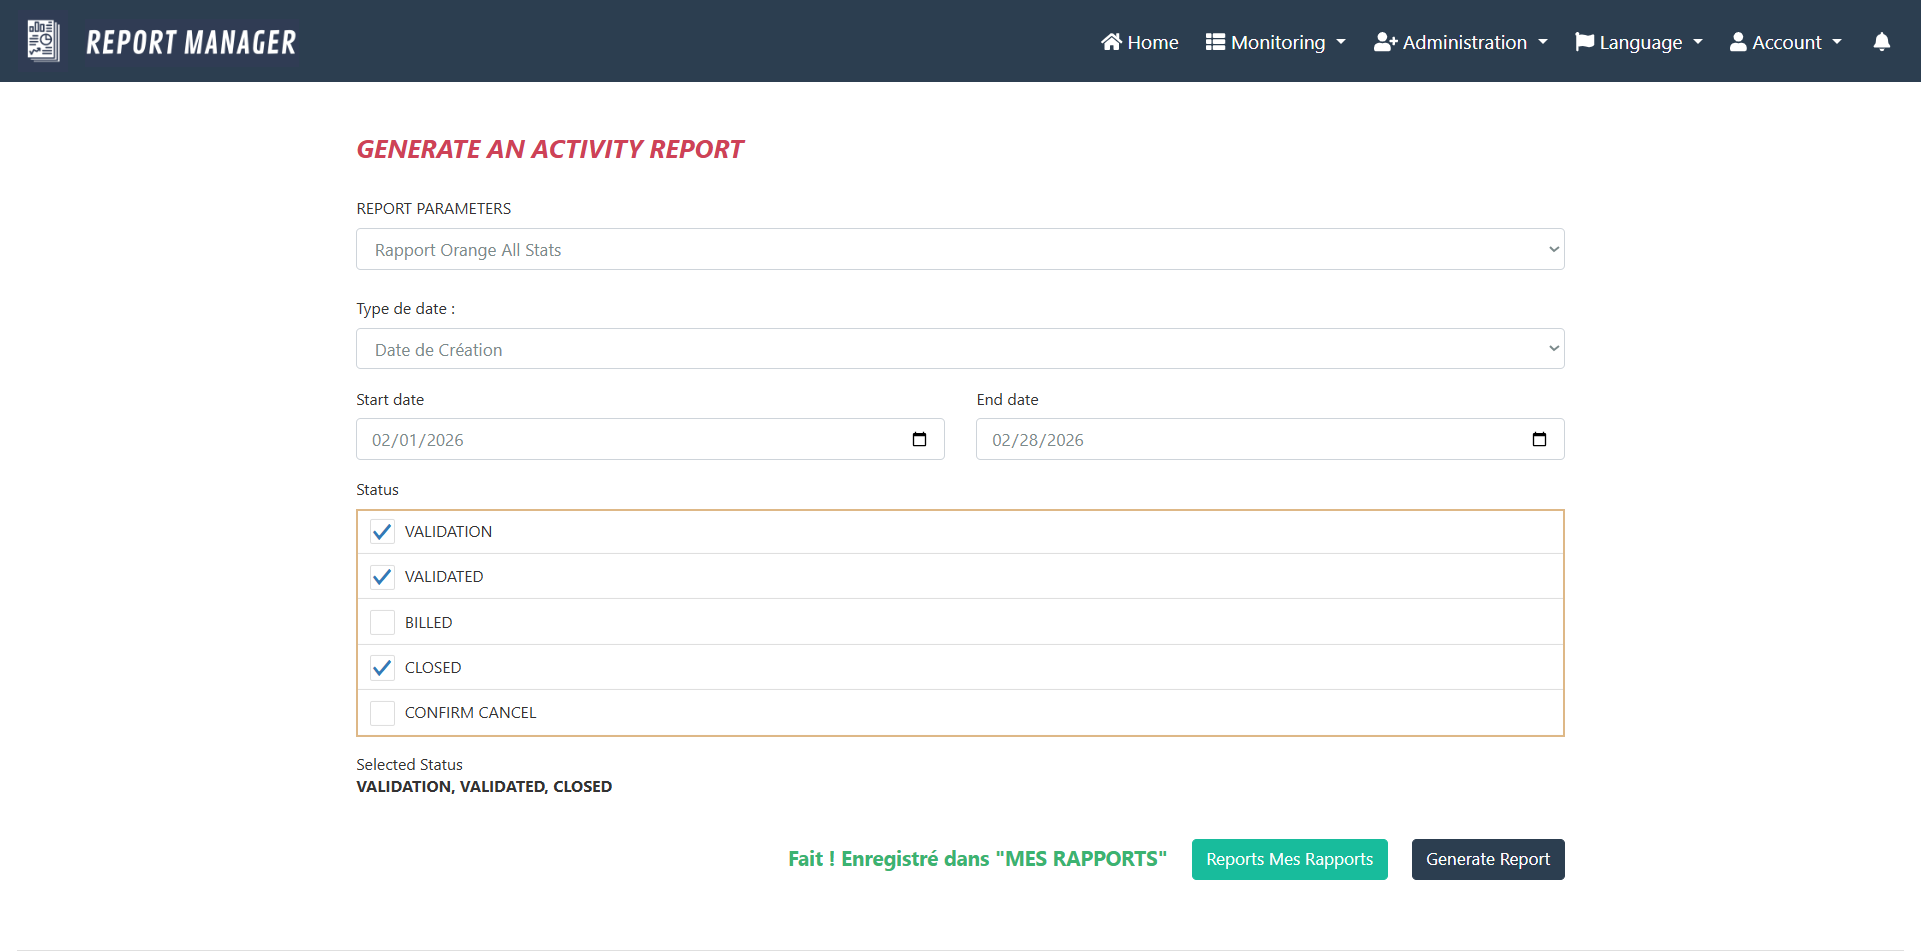
\includegraphics[width=1\textwidth]{conf2.png}
File configuration for a custom Excel report template with dynamic column mapping
}}
\caption{Sprint 5 File Configuration}
\label{fig:sprint5_file_config}
\end{figure}


\begin{figure}[H]
\centering
\fbox{\parbox{1\textwidth}{
\centering
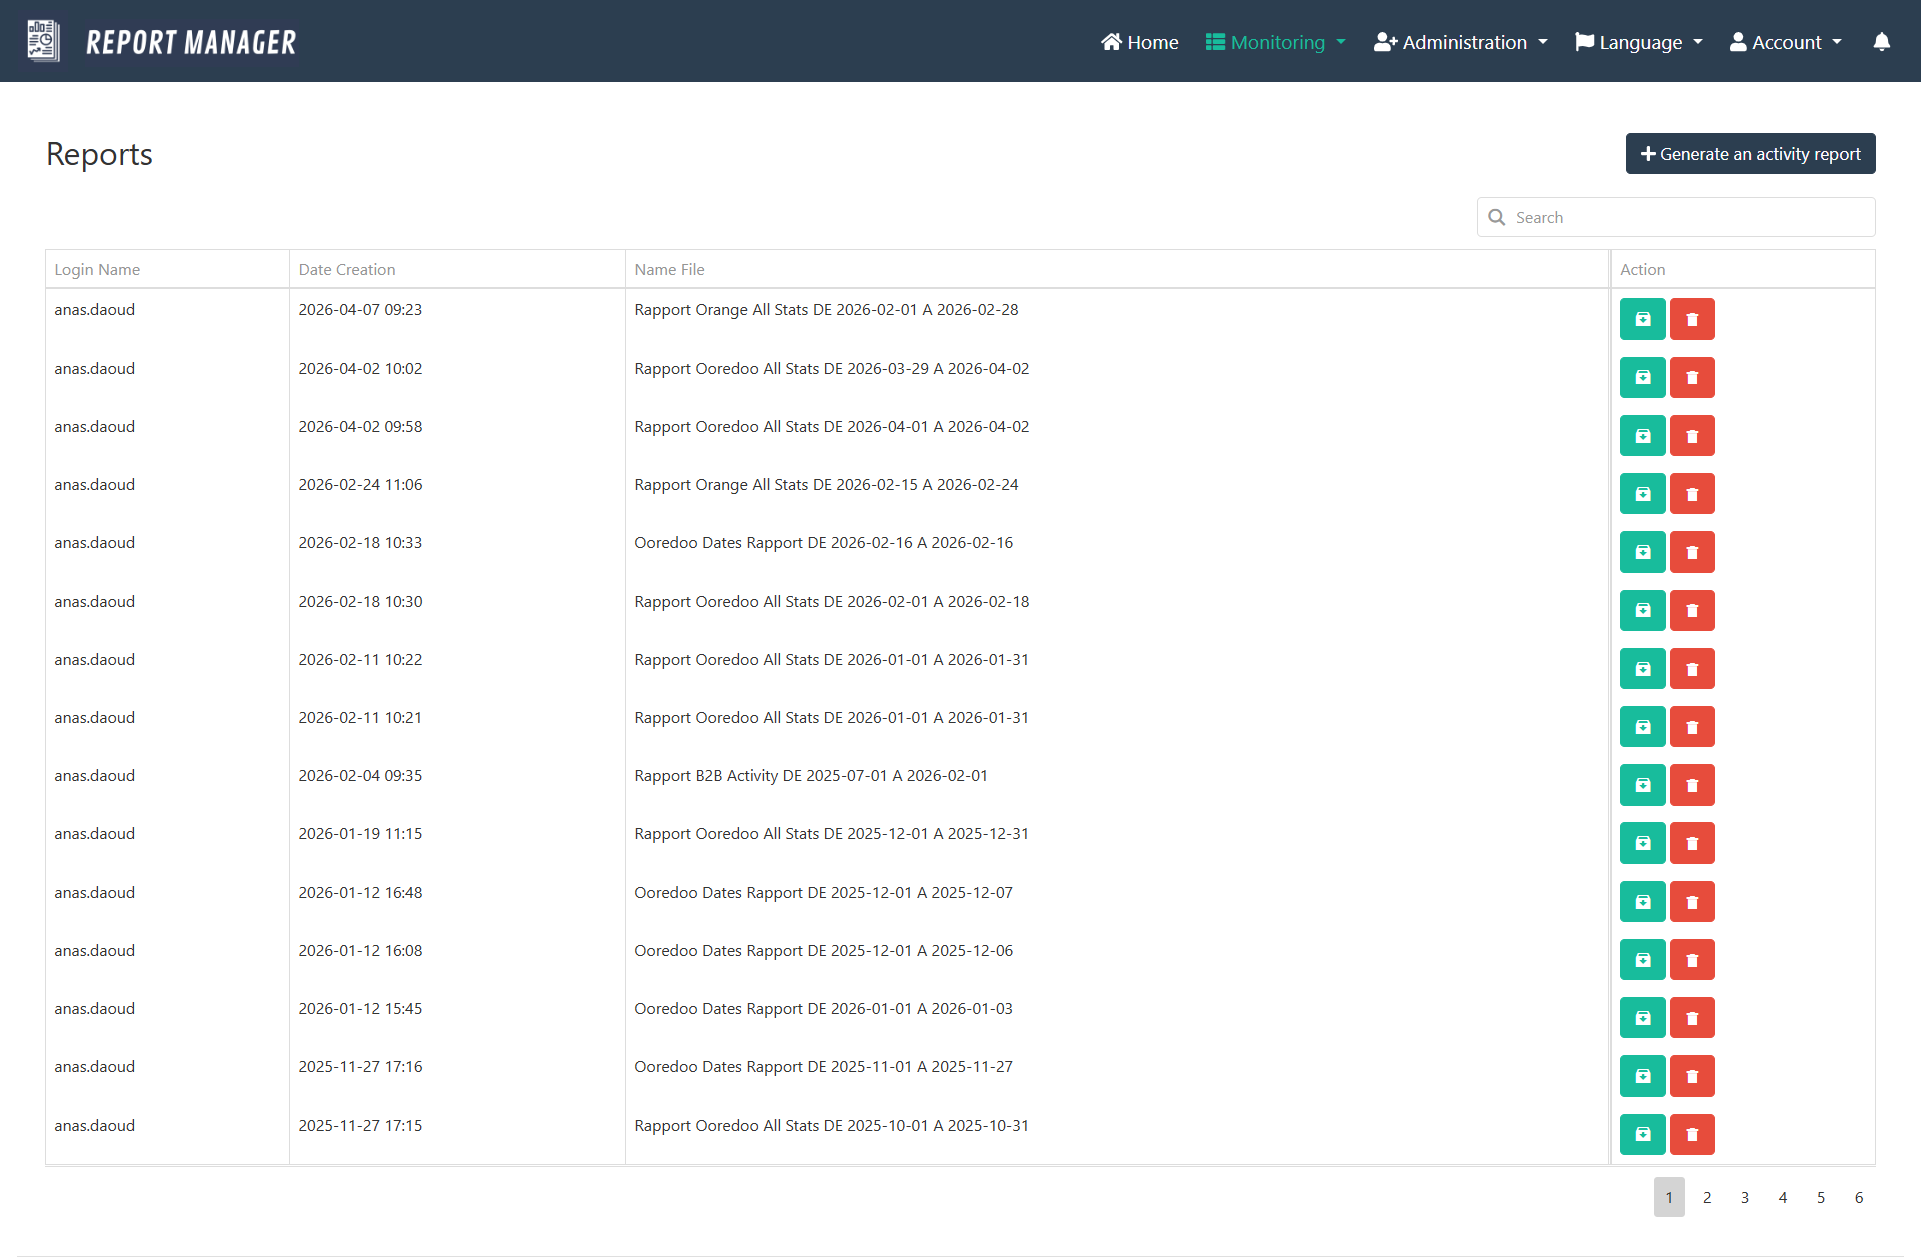
\includegraphics[width=1\textwidth]{conf3.png}
List of Generated Activity Report Excel Files with timestamps and download links
}}
\caption{Sprint 5 List of Generated Reports Links}
\label{fig:sprint5_generated}
\end{figure}


\begin{figure}[H]
\centering
\fbox{\parbox{1\textwidth}{
\centering
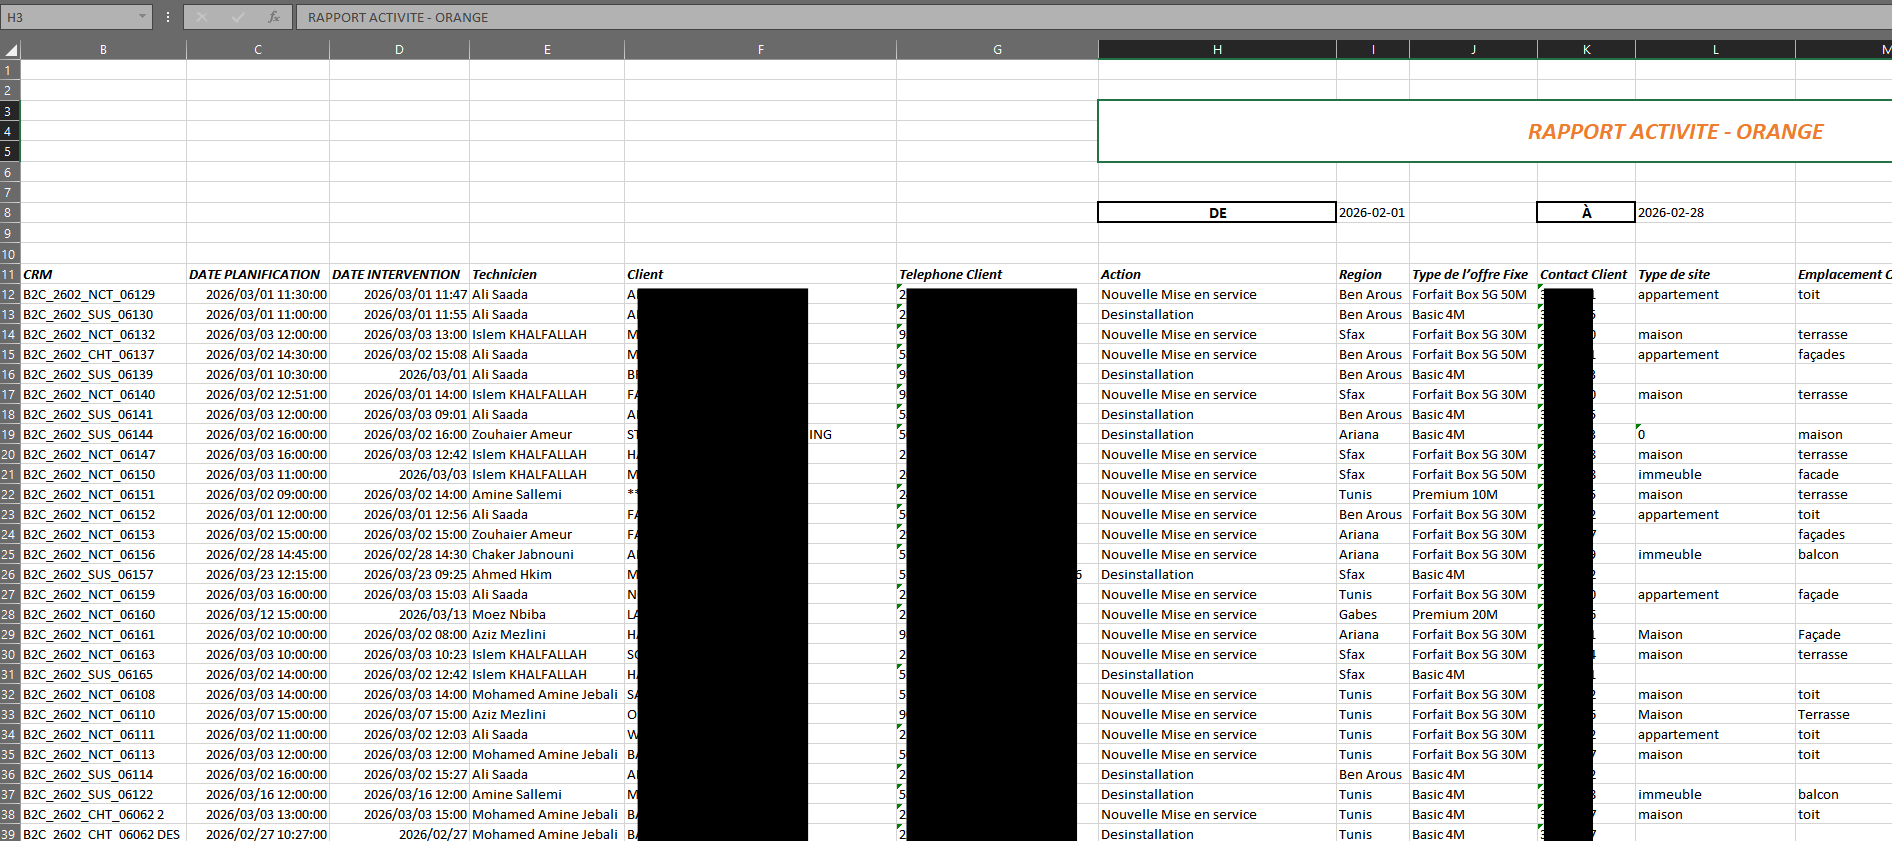
\includegraphics[width=1\textwidth]{conf4.png}
Example of a generated Excel report with dynamic data population and formatting
}}
\caption{Sprint 5 Generated Report}
\label{fig:sprint5_generated}
\end{figure}

\subsection{Key Achievements}

\begin{itemize}
\item Dynamic and reusable Excel reporting system.
\item Template-based column configuration to align with organizational standards.
\item Efficient data retrieval and aggregation for high-volume intervention records.
\item Automated archival process maintaining database performance.
\item System monitoring enabling proactive detection of performance bottlenecks.
\end{itemize}
\section{System Metrics and Monitoring}

The system includes comprehensive monitoring integration:

\begin{table}[H]
\centering
\caption{Key Monitored Metrics}
\label{tab:metrics}
\begin{tabularx}{\textwidth}{|l|X|}
\hline
\textbf{Metric} & \textbf{Description} \\
\hline
HTTP Requests & Total requests, response times by endpoint \\
\hline
Database Queries & Query count, slow query detection \\
\hline
Cache Hit Rate & Cache effectiveness metrics \\
\hline
Disk Space & File storage and backup monitoring \\
\hline
Memory Usage & Heap usage, garbage collection metrics \\
\hline
Failed Requests & Error rates and error type distribution \\
\hline
\end{tabularx}
\end{table}

\begin{figure}[H]
\centering
\fbox{\parbox{1\textwidth}{
\centering
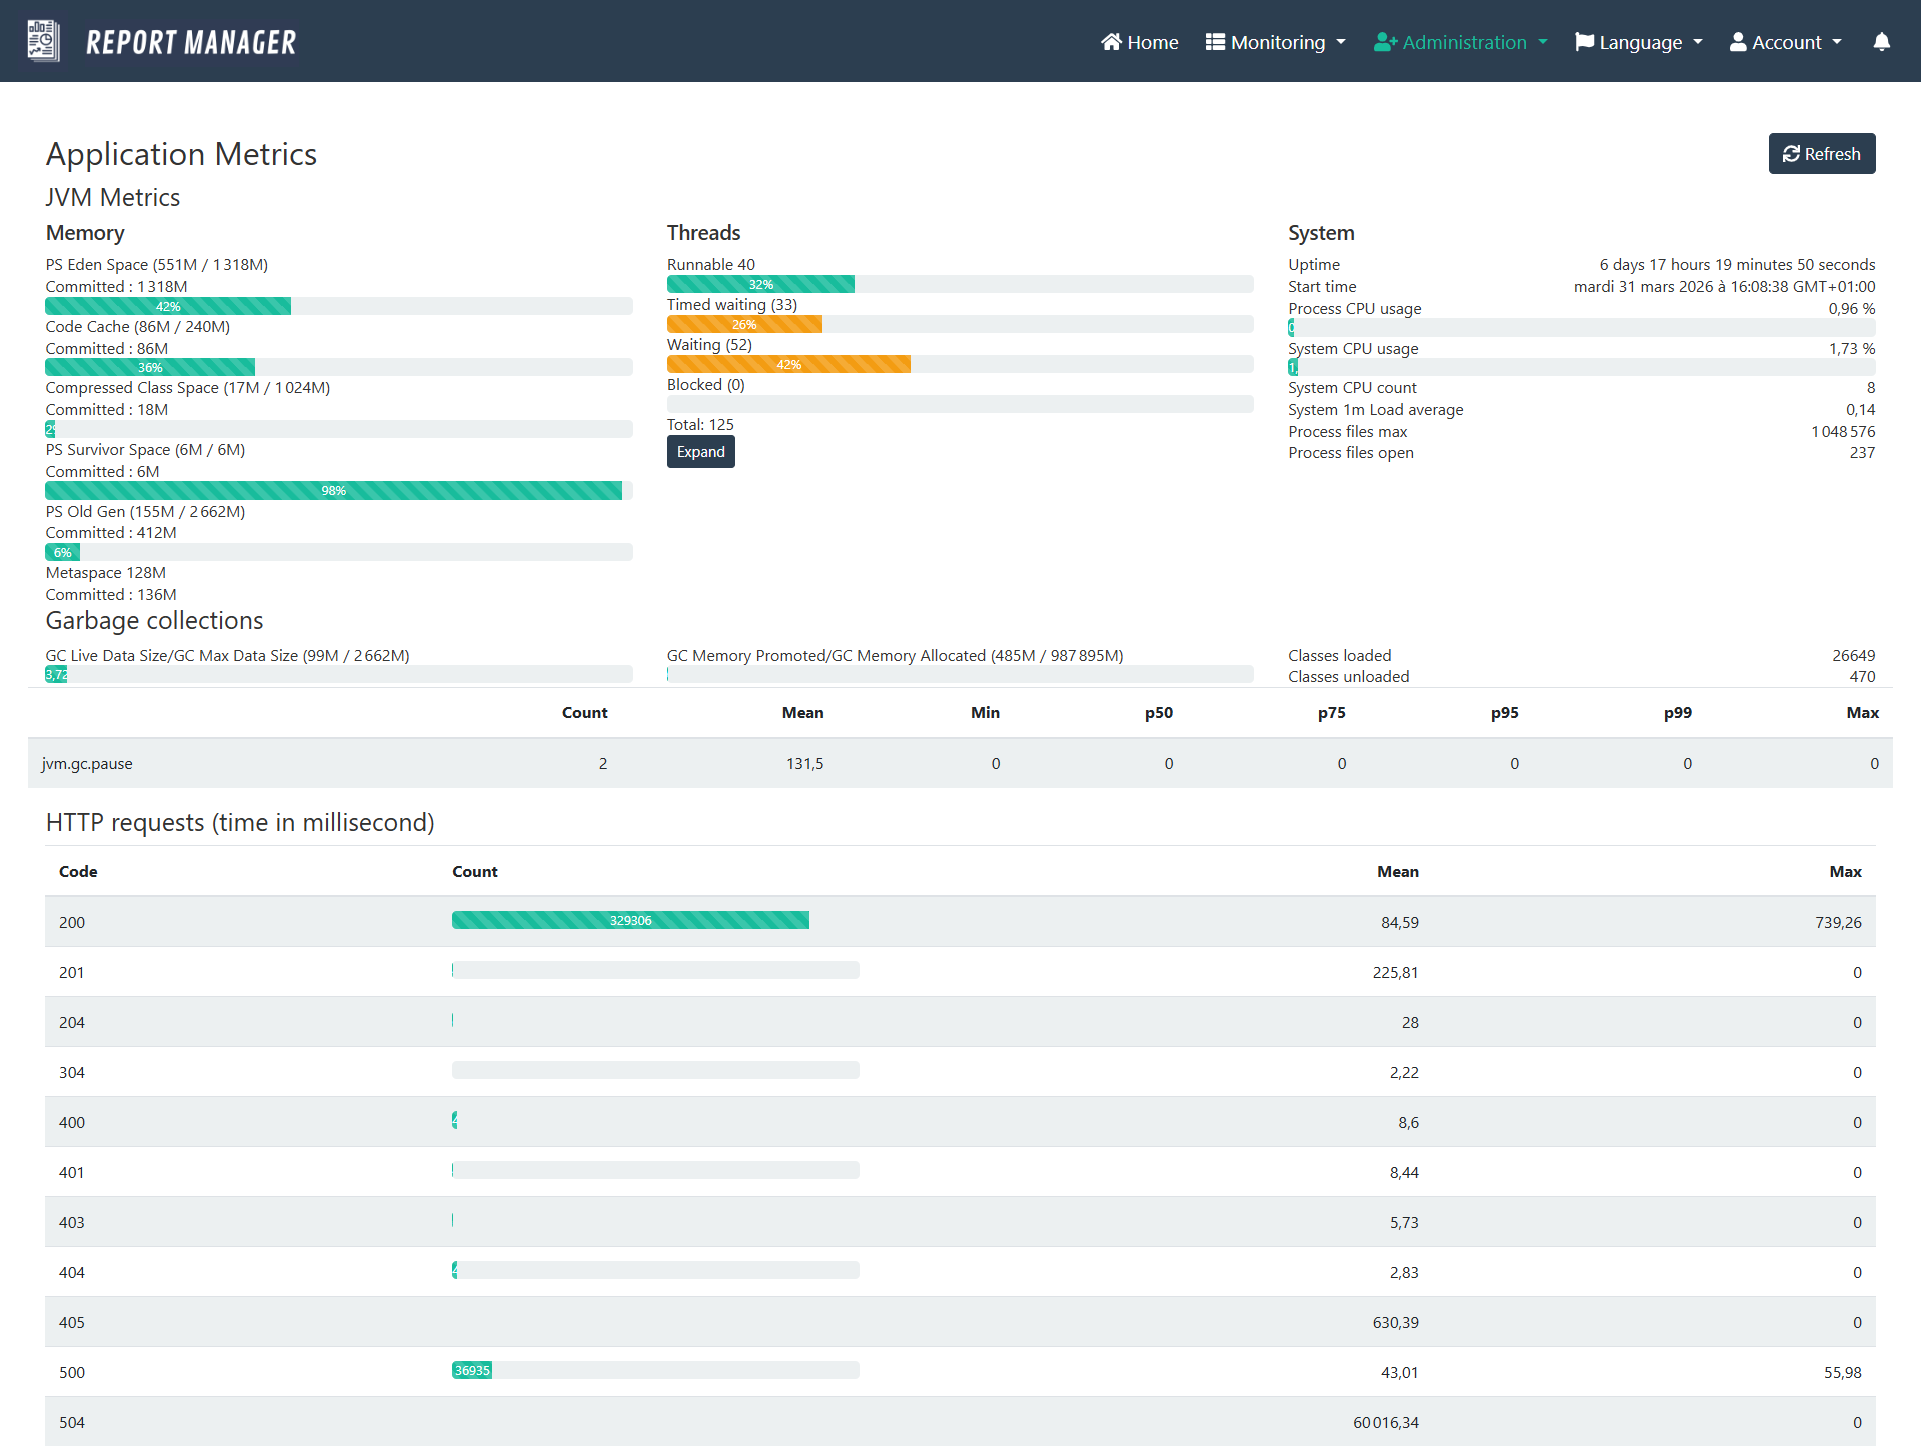
\includegraphics[width=1\textwidth]{mzt.png}
System monitoring dashboard illustrating key performance metrics
}}
\caption{Sprint 5 Monitoring Dashboard}
\label{fig:sprint5_monitoring}
\end{figure}

\section{Conclusion}

Sprint 5 successfully completed the development of the Report Manager system with comprehensive reporting capabilities and production-ready optimization. The Excel report generation enables organizational decision-making and data analysis. Performance optimization ensures the system scales effectively with growing data volumes.

Key achievements:
\begin{itemize}
\item Comprehensive Excel report generation with custom templates
\item Configurable report templates for organizational standards
\item Automated archival strategy for database optimization
\item Query optimization and intelligent caching
\item System monitoring and health metrics
\end{itemize}

The complete system now provides:
\begin{enumerate}
\item \textbf{Foundation Phase:} Authentication, database, API infrastructure
\item \textbf{Core Functionality:} Intervention management and form templates
\item \textbf{Evidence Management:} File uploads and geolocation tracking
\item \textbf{Quality Assurance:} Approval workflows and status management
\item \textbf{Business Analytics:} Advanced reporting and system optimization
\end{enumerate}

All five development sprints have been successfully completed, delivering a fully functional, production-ready intervention management system.


% General Conclusion
% Conclusion Chapter

\chapter*{Conclusion}
\addcontentsline{toc}{chapter}{Conclusion}

\section*{Overview}

The Report Manager (RM) project represents a comprehensive, multi-tier software engineering effort spanning five development sprints. This document has detailed the complete journey from initial conceptualization through production-ready implementation, encompassing architectural design, requirements specification, and technical realization across backend, frontend, and mobile platforms.

\section*{Achievements}

\subsection*{Technical Deliverables}

The project successfully delivered five core system features:

\begin{enumerate}
\item \textbf{Foundation Infrastructure:} JWT-based authentication, API gateway, core database schema, and development environment setup providing secure, scalable infrastructure.

\item \textbf{Intervention Management:} Dynamic form templates, JSONB-based data structures, comprehensive CRUD operations, and technician mobile interface enabling efficient work order management.

\item \textbf{Evidence Capture:} File upload/download, automatic image optimization, geolocation tracking, and offline file queuing supporting accountability and documentation.

\item \textbf{Quality Assurance:} Status management, approval workflows, rejection feedback, and audit trails enabling supervisory control and continuous improvement.

\item \textbf{Business Analytics:} Excel report generation, custom templates, intelligent archival, and system optimization providing organizational intelligence and performance.
\end{enumerate}

\subsection*{Technology Stack Mastery}

The project demonstrates proficiency across enterprise technologies:

\textbf{Backend:}
\begin{itemize}
\item Spring Boot 2.7.x with Spring Security for authentication
\item JHipster framework for rapid microservice development
\item Spring Data JPA with custom repositories
\item PostgreSQL 15 with JSONB for flexible data structures
\item Scheduled tasks and background job processing
\end{itemize}

\textbf{Frontend:}
\begin{itemize}
\item Angular 10 with TypeScript
\item Bootstrap and CoreUI for UI components
\item Reactive forms and real-time updates
\item Component-based architecture
\end{itemize}

\textbf{Mobile:}
\begin{itemize}
\item Flutter 3.7.x for cross-platform development
\item BLoC pattern for state management
\item Firebase Cloud Messaging for notifications
\item Local storage and offline functionality
\end{itemize}

\textbf{Infrastructure:}
\begin{itemize}
\item Docker containerization and Docker Compose orchestration
\item PostgreSQL database administration
\item File storage and management
\item Cloud deployment strategies
\end{itemize}

\section*{Software Engineering Excellence}

\subsection*{SCRUM Methodology Application}

The project exemplifies professional SCRUM practices:

\begin{itemize}
\item \textbf{Sprint Planning:} Five two-week sprints with clear objectives
\item \textbf{User Stories:} 25 comprehensive user stories totaling 225 story points
\item \textbf{Backlog Management:} Iterative refinement and prioritization
\item \textbf{Velocity Tracking:} Consistent 45-point velocities across sprints
\item \textbf{Retrospectives:} Continuous improvement based on team feedback
\end{itemize}

\subsection*{Architecture and Design Patterns}

The system implements industry-standard patterns:

\begin{itemize}
\item \textbf{Microservices:} Independent services with clear boundaries
\item \textbf{API Gateway:} Centralized request routing and security
\item \textbf{Repository Pattern:} Data access abstraction and testability
\item \textbf{Service Layer:} Business logic encapsulation
\item \textbf{State Management:} BLoC pattern for mobile state handling
\item \textbf{Observer Pattern:} Real-time notifications and event handling
\end{itemize}

\subsection*{Security and Authorization}

Comprehensive security implementation:

\begin{itemize}
\item JWT token-based authentication with refresh mechanisms
\item Role-Based Access Control (RBAC) with fine-grained permissions
\item @PreAuthorize decorators for endpoint protection
\item Secure password hashing and validation
\item Input validation and SQL injection prevention
\end{itemize}

\subsection*{Testing and Quality Assurance}

Rigorous testing approach across all layers:

\begin{itemize}
\item \textbf{Unit Tests:} Service and component-level tests
\item \textbf{Integration Tests:} API endpoint validation
\item \textbf{UI Tests:} Angular component testing
\item \textbf{End-to-End Tests:} Complete user workflows
\item \textbf{Performance Tests:} Load testing and optimization
\end{itemize}

\section*{Key Technical Innovations}

\subsection*{JSONB Data Flexibility}

Leveraging PostgreSQL's JSONB capability for:
\begin{itemize}
\item Dynamic form field configuration
\item Flexible intervention data structures
\item Self-documenting data without schema changes
\item Complex queries on semi-structured data
\end{itemize}

\subsection*{Offline-First Mobile Architecture}

The Flutter application implements:
\begin{itemize}
\item Local database for offline form completion
\item Queue-based file uploads
\item Automatic synchronization when connectivity restored
\item User experience continuity
\end{itemize}

\subsection*{Performance Optimization}

Systematic optimization at multiple levels:
\begin{itemize}
\item Eager loading with JOIN FETCH to reduce N+1 queries
\item Caching strategy for frequently accessed data
\item Database indexing on search columns
\item Image compression before storage
\item Automated archival of old data
\end{itemize}

\section*{Project Metrics}

\begin{table}[H]
\centering
\caption{Project Statistics}
\label{tab:project_metrics}
\begin{tabularx}{\textwidth}{|l|r|}
\hline
\textbf{Metric} & \textbf{Value} \\
\hline
Total Development Sprints & 5 \\
\hline
Total Story Points & 225 \\
\hline
User Stories Delivered & 25 \\
\hline
Development Duration & 10 weeks \\
\hline
Team Size & 3-5 developers \\
\hline
Estimated Lines of Code & 15,000+ \\
\hline
Database Tables & 30+ \\
\hline
API Endpoints & 50+ \\
\hline
Mobile Screens & 15+ \\
\hline
Angular Components & 20+ \\
\hline
\end{tabularx}
\end{table}

\section*{Documentation Completeness}

This report provides:

\begin{enumerate}
\item \textbf{Requirements Documentation:} Comprehensive stakeholder analysis, functional and non-functional requirements
\item \textbf{Architecture Documentation:} Physical, logical, and microservices architecture diagrams
\item \textbf{Design Documentation:} UML class diagrams, sequence diagrams, state diagrams
\item \textbf{Implementation Documentation:} Code samples, configuration details, integration points
\item \textbf{Testing Documentation:} Test strategies, test cases, coverage metrics
\item \textbf{Deployment Documentation:} Docker configuration, environment setup, deployment procedures
\end{enumerate}

\section*{Lessons Learned}

\subsection*{Technical Insights}

\begin{itemize}
\item JSONB provides excellent flexibility but requires careful schema documentation
\item BLoC pattern effectively manages mobile state complexity
\item Proper indexing and eager loading are critical for query performance
\item Offline-first architecture significantly improves user experience on unreliable connections
\end{itemize}

\subsection*{Process Insights}

\begin{itemize}
\item Sprint planning with realistic velocity estimates enables consistent delivery
\item Comprehensive user story acceptance criteria prevent scope creep
\item Regular code reviews catch architectural issues early
\item Automated testing provides confidence in refactoring and optimization
\end{itemize}

\section*{Future Recommendations}

\subsection*{Short-term Enhancements (0-3 months)}

\begin{enumerate}
\item Implement advanced search with Elasticsearch for large datasets
\item Add audit logging for compliance and forensics
\item Implement role-based view customization
\item Add batch operation capabilities for supervisor workflows
\item Enhance mobile offline capabilities with background sync
\end{enumerate}

\subsection*{Medium-term Improvements (3-6 months)}

\begin{enumerate}
\item Implement real-time collaboration features
\item Add advanced analytics and business intelligence dashboards
\item Implement automated quality assurance scoring
\item Add multi-language support for international operations
\item Implement predictive maintenance recommendations
\end{enumerate}

\subsection*{Long-term Vision (6-12 months)}

\begin{enumerate}
\item Machine learning for scheduling optimization
\item IoT integration for equipment tracking
\item Advanced geofencing for location-based services
\item Mobile augmented reality for technical documentation
\item Blockchain integration for immutable intervention records
\end{enumerate}

\section*{Professional Growth}

This project provided comprehensive experience in:

\begin{itemize}
\item Full-stack development across Java, TypeScript, and Dart
\item Enterprise architecture and microservices design
\item Complex database design with both relational and semi-structured data
\item Mobile-first development with Flutter
\item SCRUM methodology and agile practices
\item CI/CD pipeline implementation
\item Cloud deployment and containerization
\item Team collaboration and documentation
\end{itemize}

\section*{Final Remarks}

The Report Manager project demonstrates the successful execution of a complex, multi-tier software engineering initiative. The system is production-ready, scalable, and maintainable, providing significant value to the host organization. The comprehensive documentation ensures knowledge transfer and future maintenance.

The five development sprints successively built upon each preceding sprint, creating a cohesive system where each component integrates seamlessly with others. The project exemplifies professional software engineering practices, from initial requirements analysis through final deployment and monitoring.

The Report Manager system is now ready for deployment and will enable the host organization to significantly improve operational efficiency, quality assurance, and decision-making through comprehensive intervention management and analytics.

\vskip 1cm

\noindent
\textbf{Date:} \today

\noindent
\textbf{Status:} Development Complete, Ready for Production Deployment


% Appendices
\appendix
% Appendix A: Code Samples

\chapter{Code Samples}

\section{Backend Code Samples}

\subsection{JWT Authentication Implementation}

\begin{lstlisting}
// JwtAuthenticationFilter.java
@Component
public class JwtAuthenticationFilter extends OncePerRequestFilter {

    private final TokenProvider tokenProvider;
    private final UserRepository userRepository;

    @Override
    protected void doFilterInternal(HttpServletRequest request,
                                    HttpServletResponse response,
                                    FilterChain filterChain)
            throws ServletException, IOException {

        final String requestTokenHeader = request.getHeader("Authorization");

        String username = null;
        String jwtToken = null;

        if (requestTokenHeader != null && requestTokenHeader.startsWith("Bearer ")) {
            jwtToken = requestTokenHeader.substring(7);
            try {
                username = tokenProvider.getUsernameFromToken(jwtToken);
            } catch (IllegalArgumentException e) {
                logger.error("Unable to get JWT Token");
            } catch (ExpiredJwtException e) {
                logger.error("JWT Token has expired");
            }
        }

        if (username != null && SecurityContextHolder.getContext().getAuthentication() == null) {
            UserDetails userDetails = userRepository.findByLogin(username);

            if (tokenProvider.validateToken(jwtToken, userDetails)) {
                UsernamePasswordAuthenticationToken authenticationToken =
                    new UsernamePasswordAuthenticationToken(
                        userDetails, null, userDetails.getAuthorities());

                authenticationToken.setDetails(
                    new WebAuthenticationDetailsSource().buildDetails(request));

                SecurityContextHolder.getContext().setAuthentication(authenticationToken);
            }
        }
        filterChain.doFilter(request, response);
    }
}
\end{lstlisting}

\subsection{JSONB Entity Mapping}

\begin{lstlisting}
// RapportRequest.java - JSONB field mapping
@Entity
@Table(name = "rapport_request")
@TypeDefs({
    @TypeDef(name = "jsonb", typeClass = JsonBinaryType.class),
})
public class RapportRequest extends AbstractAuditingEntity {

    @Type(type = "jsonb")
    @Column(columnDefinition = "jsonb")
    private Object reportLineData;

    @Type(type = "jsonb")
    @Column(columnDefinition = "jsonb")
    private Object filedefinition;

    // getters and setters
}
\end{lstlisting}

\section{Frontend Code Samples}

\subsection{Angular Authentication Service}

\begin{lstlisting}
// auth.service.ts
@Injectable({
  providedIn: 'root'
})
export class AuthService {

  private apiUrl = environment.apiUrl + '/authenticate';
  private tokenKey = 'authToken';

  constructor(private http: HttpClient, private router: Router) {}

  login(credentials: {username: string, password: string}): Observable<any> {
    return this.http.post(this.apiUrl, credentials).pipe(
      tap((response: any) => {
        if (response.token) {
          localStorage.setItem(this.tokenKey, response.token);
        }
      }),
      catchError(error => {
        console.error('Login error:', error);
        return throwError(error);
      })
    );
  }

  logout(): void {
    localStorage.removeItem(this.tokenKey);
    this.router.navigate(['/login']);
  }

  getToken(): string | null {
    return localStorage.getItem(this.tokenKey);
  }

  isAuthenticated(): boolean {
    const token = this.getToken();
    return !!token && !this.isTokenExpired(token);
  }

  private isTokenExpired(token: string): boolean {
    // Implement token expiration check
    return false;
  }
}
\end{lstlisting}

\section{Mobile Code Samples}

\subsection{Flutter BLoC Implementation}

\begin{lstlisting}
// login_bloc.dart
class LoginBloc extends Bloc<LoginEvent, LoginState> {
  final LoginRepository loginRepository;

  LoginBloc(this.loginRepository) : super(LoginInitial()) {
    on<LoginRequested>(_onLoginRequested);
  }

  Future<void> _onLoginRequested(
    LoginRequested event,
    Emitter<LoginState> emit,
  ) async {
    emit(LoginLoading());
    try {
      final response = await loginRepository.login(
        event.email,
        event.password,
      );

      // Store token securely
      await _secureStorage.write(
        key: 'jwt_token',
        value: response.token,
      );

      emit(LoginSuccess(user: response.user));
    } catch (e) {
      emit(LoginFailure(error: e.toString()));
    }
  }
}
\end{lstlisting}

\subsection{Dynamic Form Widget}

\begin{lstlisting}
// dynamic_form_widget.dart
class DynamicFormWidget extends StatefulWidget {
  final Map<String, dynamic> formSchema;
  final Function(Map<String, dynamic>) onFormChanged;

  const DynamicFormWidget({
    Key? key,
    required this.formSchema,
    required this.onFormChanged,
  }) : super(key: key);

  @override
  State<DynamicFormWidget> createState() => _DynamicFormWidgetState();
}

class _DynamicFormWidgetState extends State<DynamicFormWidget> {
  final Map<String, dynamic> _formData = {};

  @override
  Widget build(BuildContext context) {
    return ListView.builder(
      itemCount: widget.formSchema['fields']?.length ?? 0,
      itemBuilder: (context, index) {
        final field = widget.formSchema['fields'][index];
        return _buildFormField(field);
      },
    );
  }

  Widget _buildFormField(Map<String, dynamic> field) {
    final fieldType = field['type'];
    final fieldName = field['name'];
    final label = field['label'];

    switch (fieldType) {
      case 'text':
        return TextFormField(
          decoration: InputDecoration(labelText: label),
          onChanged: (value) {
            _formData[fieldName] = value;
            widget.onFormChanged(_formData);
          },
        );
      case 'number':
        return TextFormField(
          decoration: InputDecoration(labelText: label),
          keyboardType: TextInputType.number,
          onChanged: (value) {
            _formData[fieldName] = num.tryParse(value);
            widget.onFormChanged(_formData);
          },
        );
      // Add more field types as needed
      default:
        return const SizedBox.shrink();
    }
  }
}
\end{lstlisting}
% Appendix B: Detailed Diagrams

\chapter{Detailed Diagrams}

\section{System Architecture Diagrams}

\subsection{Complete System Architecture}

\begin{figure}[H]
\centering
\begin{tikzpicture}[node distance=2cm, auto]
  % Define styles
  \tikzstyle{component}=[rectangle, draw=black, fill=blue!10, text width=3cm, text centered, minimum height=1cm]
  \tikzstyle{external}=[rectangle, draw=black, fill=green!10, text width=3cm, text centered, minimum height=1cm]
  \tikzstyle{database}=[cylinder, draw=black, fill=red!10, text width=3cm, text centered, minimum height=1cm, shape border rotate=90]
  \tikzstyle{arrow}=[->, thick]

  % Mobile Layer
  \node[component] (mobile) {Flutter Mobile App};

  % Web Layer
  \node[component, below of=mobile] (web) {Angular Web App};

  % API Gateway
  \node[component, below of=web] (gateway) {JHipster API Gateway};

  % Microservices
  \node[component, left of=gateway, xshift=-3cm] (auth) {Auth Service};
  \node[component, below of=auth] (user) {User Service};
  \node[component, right of=gateway, xshift=3cm] (report) {Report Service};
  \node[component, below of=report] (template) {Template Service};

  % Database
  \node[database, below of=user, yshift=-1cm] (db) {PostgreSQL Database};

  % External Services
  \node[external, right of=report, xshift=2cm] (firebase) {Firebase Cloud Messaging};

  % Connections
  \draw[arrow] (mobile) -- (gateway);
  \draw[arrow] (web) -- (gateway);
  \draw[arrow] (gateway) -- (auth);
  \draw[arrow] (gateway) -- (report);
  \draw[arrow] (auth) -- (db);
  \draw[arrow] (user) -- (db);
  \draw[arrow] (report) -- (db);
  \draw[arrow] (template) -- (db);
  \draw[arrow] (report) -- (firebase);
\end{tikzpicture}
\caption{Complete RM System Architecture}
\label{fig:system_architecture}
\end{figure}

\subsection{Database Schema Diagram}

\begin{figure}[H]
\centering
\begin{tikzpicture}[node distance=1.5cm, auto]
  % Define styles
  \tikzstyle{table}=[rectangle, draw=black, fill=blue!5, text width=2.5cm, text centered, minimum height=0.8cm]
  \tikzstyle{fk}=[->, thick, color=red]

  % Tables
  \node[table] (user) {jhi\_user};
  \node[table, right of=user] (authority) {jhi\_authority};
  \node[table, below of=user] (client) {client};
  \node[table, right of=client] (company) {company};
  \node[table, below of=client] (project) {projet};
  \node[table, right of=project] (template) {rapport\_template};
  \node[table, below of=template] (request) {rapport\_request};
  \node[table, right of=request] (status) {status};
  \node[table, below of=request] (files) {files};

  % Relationships
  \draw[fk] (user) -- (authority);
  \draw[fk] (project) -- (client);
  \draw[fk] (project) -- (company);
  \draw[fk] (template) -- (project);
  \draw[fk] (request) -- (template);
  \draw[fk] (request) -- (status);
  \draw[fk] (files) -- (request);
\end{tikzpicture}
\caption{Database Entity-Relationship Diagram}
\label{fig:database_schema}
\end{figure}

\section{Use Case Diagrams}

\subsection{Complete System Use Case Diagram}

\begin{figure}[H]
\centering
\begin{tikzpicture}[node distance=2cm, auto]
  % Define styles
  \tikzstyle{actor}=[rectangle, draw=black, fill=yellow!20, text width=2cm, text centered, minimum height=1cm]
  \tikzstyle{usecase}=[ellipse, draw=black, fill=green!10, text width=2.5cm, text centered, minimum height=0.8cm]
  \tikzstyle{arrow}=[->, thick]

  % Actors
  \node[actor] (technician) {Field Technician};
  \node[actor, below of=technician] (supervisor) {Project Supervisor};
  \node[actor, below of=supervisor] (coordinator) {Project Coordinator};
  \node[actor, below of=coordinator] (admin) {System Administrator};

  % Use Cases
  \node[usecase, right of=technician, xshift=3cm] (login) {User Authentication};
  \node[usecase, below of=login] (view) {View Interventions};
  \node[usecase, below of=view] (fill) {Fill Dynamic Forms};
  \node[usecase, below of=fill] (submit) {Submit Interventions};
  \node[usecase, right of=coordinator, xshift=3cm] (create) {Create Templates};
  \node[usecase, below of=create] (manage) {Manage Interventions};
  \node[usecase, below of=manage] (reports) {Generate Reports};

  % Relationships
  \draw[arrow] (technician) -- (login);
  \draw[arrow] (technician) -- (view);
  \draw[arrow] (technician) -- (fill);
  \draw[arrow] (technician) -- (submit);
  \draw[arrow] (coordinator) -- (create);
  \draw[arrow] (coordinator) -- (manage);
  \draw[arrow] (supervisor) -- (reports);
  \draw[arrow] (admin) -- (login);
\end{tikzpicture}
\caption{Complete System Use Case Diagram}
\label{fig:use_case_diagram}
\end{figure}

\section{Sequence Diagrams}

\subsection{Authentication Flow Sequence Diagram}

\begin{figure}[H]
\centering
\begin{lstlisting}
\newthread{user}{User}
\newthread{client}{Client App}
\newthread{gateway}{API Gateway}
\newthread{auth}{Auth Service}
\newthread{db}{Database}

\begin{call}{user}{client}{Enter credentials}
\end{call}

\begin{call}{client}{gateway}{POST /api/authenticate}
\end{call}

\begin{call}{gateway}{auth}{validateCredentials()}
\end{call}

\begin{call}{auth}{db}{findByLogin()}
\end{call}

\begin{callself}{db}{auth}{Return user}
\end{callself}

\begin{callself}{auth}{auth}{generateToken()}
\end{callself}

\begin{callself}{auth}{gateway}{Return token}
\end{callself}

\begin{callself}{gateway}{client}{200 OK + token}
\end{callself}

\begin{callself}{client}{client}{Store token}
\end{callself}
\end{lstlisting}
\caption{Authentication Flow Sequence Diagram}
\label{fig:auth_sequence}
\end{figure}

\section{State Diagrams}

\subsection{Intervention Lifecycle State Diagram}

\begin{figure}[H]
\centering
\begin{tikzpicture}[node distance=2cm, auto, >=stealth]
  % Define styles
  \tikzstyle{state}=[circle, draw=black, fill=blue!20, text width=2cm, text centered, minimum height=1cm]
  \tikzstyle{transition}=[->, thick]

  % States
  \node[state] (planned) {PLANNED};
  \node[state, right of=planned] (executed) {EXECUTED};
  \node[state, right of=executed] (validation) {PENDING\\VALIDATION};
  \node[state, right of=validation] (approved) {APPROVED};
  \node[state, below of=approved, yshift=-1cm] (archived) {ARCHIVED};
  \node[state, below of=planned, yshift=-1cm] (cancelled) {CANCELLED};
  \node[state, below of=validation, yshift=-1cm] (rejected) {REJECTED};

  % Transitions
  \draw[transition] (planned) -- node[above] {submit} (executed);
  \draw[transition] (planned) -- node[left] {cancel} (cancelled);
  \draw[transition] (executed) -- node[above] {submit} (validation);
  \draw[transition] (validation) -- node[above] {approve} (approved);
  \draw[transition] (validation) -- node[below] {reject} (rejected);
  \draw[transition] (approved) -- node[right] {auto archive} (archived);
  \draw[transition] (rejected) -- node[left] {resubmit} (executed);
\end{tikzpicture}
\caption{Intervention Lifecycle State Diagram}
\label{fig:intervention_states}
\end{figure}
% Appendix C: Testing Documentation

\chapter{Testing Documentation}

\section{Testing Strategy}

The RM project implements a comprehensive testing strategy that encompasses unit testing, integration testing, end-to-end testing, and performance testing. The testing approach follows test-driven development (TDD) principles and ensures code quality throughout the development lifecycle.

\subsection{Testing Pyramid}

The project follows the testing pyramid approach with the following distribution:
\begin{itemize}
\item \textbf{Unit Tests (70\%):} Testing individual components and methods in isolation
\item \textbf{Integration Tests (20\%):} Testing component interactions and API endpoints
\item \textbf{End-to-End Tests (10\%):} Testing complete user workflows
\end{itemize}

\section{Backend Testing}

\subsection{Unit Testing with JUnit}

\subsubsection{Service Layer Testing}

\begin{lstlisting}
// UserServiceTest.java
@SpringBootTest
class UserServiceTest {

    @Autowired
    private UserService userService;

    @Autowired
    private UserRepository userRepository;

    @Test
    void createUser_shouldCreateUserSuccessfully() {
        // Given
        UserDTO userDTO = new UserDTO();
        userDTO.setLogin("testuser");
        userDTO.setEmail("test@example.com");
        userDTO.setPassword("password");

        // When
        UserDTO result = userService.createUser(userDTO);

        // Then
        assertThat(result.getId()).isNotNull();
        assertThat(result.getLogin()).isEqualTo("testuser");
        assertThat(result.getEmail()).isEqualTo("test@example.com");
    }

    @Test
    void createUser_withExistingLogin_shouldThrowException() {
        // Given
        UserDTO existingUser = createTestUser("existing");
        UserDTO duplicateUser = new UserDTO();
        duplicateUser.setLogin("existing");

        // When & Then
        assertThrows(BadRequestAlertException.class, () -> {
            userService.createUser(duplicateUser);
        });
    }
}
\end{lstlisting}

\subsubsection{Controller Testing with MockMvc}

\begin{lstlisting}
// AuthControllerTest.java
@SpringBootTest
@AutoConfigureMockMvc
class AuthControllerTest {

    @Autowired
    private MockMvc mockMvc;

    @Autowired
    private UserRepository userRepository;

    @Test
    void authenticate_withValidCredentials_shouldReturnToken() throws Exception {
        // Given
        createTestUser();

        // When
        mockMvc.perform(post("/api/authenticate")
                .contentType(MediaType.APPLICATION_JSON)
                .content("{\"username\":\"test\",\"password\":\"test\"}"))
                .andExpect(status().isOk())
                .andExpect(jsonPath("$.token").exists());
    }

    @Test
    void authenticate_withInvalidCredentials_shouldReturnUnauthorized() throws Exception {
        // When
        mockMvc.perform(post("/api/authenticate")
                .contentType(MediaType.APPLICATION_JSON)
                .content("{\"username\":\"invalid\",\"password\":\"invalid\"}"))
                .andExpect(status().isUnauthorized());
    }
}
\end{lstlisting}

\subsection{Integration Testing}

\subsubsection{Database Integration Tests}

\begin{lstlisting}
// RapportRequestRepositoryTest.java
@DataJpaTest
class RapportRequestRepositoryTest {

    @Autowired
    private RapportRequestRepository repository;

    @Autowired
    private TestEntityManager entityManager;

    @Test
    void findByTechnicianId_shouldReturnRequestsForTechnician() {
        // Given
        User technician = createTestUser();
        RapportRequest request = createTestRequest(technician);

        entityManager.persist(technician);
        entityManager.persist(request);
        entityManager.flush();

        // When
        List<RapportRequest> results = repository.findByTechnicianId(technician.getId());

        // Then
        assertThat(results).hasSize(1);
        assertThat(results.get(0).getId()).isEqualTo(request.getId());
    }
}
\end{lstlisting}

\section{Frontend Testing}

\subsection{Angular Component Testing}

\begin{lstlisting}
// login.component.spec.ts
describe('LoginComponent', () => {
  let component: LoginComponent;
  let fixture: ComponentFixture<LoginComponent>;
  let authServiceSpy: jasmine.SpyObj<AuthService>;

  beforeEach(async () => {
    const spy = jasmine.createSpyObj('AuthService', ['login', 'isAuthenticated']);

    await TestBed.configureTestingModule({
      declarations: [LoginComponent],
      providers: [
        { provide: AuthService, useValue: spy }
      ]
    }).compileComponents();

    fixture = TestBed.createComponent(LoginComponent);
    component = fixture.componentInstance;
    authServiceSpy = TestBed.inject(AuthService) as jasmine.SpyObj<AuthService>;
  });

  it('should create', () => {
    expect(component).toBeTruthy();
  });

  it('should call auth service login on form submit', () => {
    const loginResponse = { token: 'test-token' };
    authServiceSpy.login.and.returnValue(of(loginResponse));

    component.loginForm.setValue({
      username: 'testuser',
      password: 'testpass'
    });

    component.onSubmit();

    expect(authServiceSpy.login).toHaveBeenCalledWith({
      username: 'testuser',
      password: 'testpass'
    });
  });
});
\end{lstlisting}

\subsection{Angular Service Testing}

\begin{lstlisting}
// auth.service.spec.ts
describe('AuthService', () => {
  let service: AuthService;
  let httpMock: HttpTestingController;

  beforeEach(() => {
    TestBed.configureTestingModule({
      imports: [HttpClientTestingModule],
      providers: [AuthService]
    });

    service = TestBed.inject(AuthService);
    httpMock = TestBed.inject(HttpTestingController);
  });

  afterEach(() => {
    httpMock.verify();
  });

  it('should login and store token', () => {
    const mockResponse = { token: 'mock-jwt-token' };

    service.login({ username: 'test', password: 'pass' }).subscribe(response => {
      expect(response.token).toBe('mock-jwt-token');
      expect(localStorage.getItem('authToken')).toBe('mock-jwt-token');
    });

    const req = httpMock.expectOne('/api/authenticate');
    expect(req.request.method).toBe('POST');
    req.flush(mockResponse);
  });
});
\end{lstlisting}

\section{Mobile Testing}

\subsection{Flutter Widget Testing}

\begin{lstlisting}
// login_screen_test.dart
void main() {
  group('LoginScreen', () {
    late MockLoginBloc mockLoginBloc;

    setUp(() {
      mockLoginBloc = MockLoginBloc();
    });

    testWidgets('renders login form', (WidgetTester tester) async {
      when(() => mockLoginBloc.state).thenReturn(LoginInitial());

      await tester.pumpWidget(
        BlocProvider<LoginBloc>.value(
          value: mockLoginBloc,
          child: MaterialApp(home: LoginScreen()),
        ),
      );

      expect(find.byType(TextFormField), findsNWidgets(2)); // email and password
      expect(find.byType(ElevatedButton), findsOneWidget);
      expect(find.text('Login'), findsOneWidget);
    });

    testWidgets('shows loading indicator when logging in', (WidgetTester tester) async {
      when(() => mockLoginBloc.state).thenReturn(LoginLoading());

      await tester.pumpWidget(
        BlocProvider<LoginBloc>.value(
          value: mockLoginBloc,
          child: MaterialApp(home: LoginScreen()),
        ),
      );

      expect(find.byType(CircularProgressIndicator), findsOneWidget);
    });

    testWidgets('navigates to home on successful login', (WidgetTester tester) async {
      when(() => mockLoginBloc.state).thenReturn(LoginSuccess(user: mockUser));

      await tester.pumpWidget(
        BlocProvider<LoginBloc>.value(
          value: mockLoginBloc,
          child: MaterialApp(home: LoginScreen()),
        ),
      );

      // Verify navigation occurred
      // (This would require a mock navigator or integration test)
    });
  });
}
\end{lstlisting}

\subsection{Flutter BLoC Testing}

\begin{lstlisting}
// login_bloc_test.dart
void main() {
  group('LoginBloc', () {
    late MockLoginRepository mockRepository;
    late LoginBloc loginBloc;

    setUp(() {
      mockRepository = MockLoginRepository();
      loginBloc = LoginBloc(mockRepository);
    });

    tearDown(() {
      loginBloc.close();
    });

    test('initial state is LoginInitial', () {
      expect(loginBloc.state, equals(LoginInitial()));
    });

    blocTest<LoginBloc, LoginState>(
      'emits [LoginLoading, LoginSuccess] when login succeeds',
      build: () {
        when(() => mockRepository.login(any(), any()))
            .thenAnswer((_) async => mockLoginResponse);
        return loginBloc;
      },
      act: (bloc) => bloc.add(LoginRequested(email: 'test@test.com', password: 'password')),
      expect: () => [
        LoginLoading(),
        LoginSuccess(user: mockUser),
      ],
      verify: (_) {
        verify(() => mockRepository.login('test@test.com', 'password')).called(1);
      },
    );

    blocTest<LoginBloc, LoginState>(
      'emits [LoginLoading, LoginFailure] when login fails',
      build: () {
        when(() => mockRepository.login(any(), any()))
            .thenThrow(Exception('Login failed'));
        return loginBloc;
      },
      act: (bloc) => bloc.add(LoginRequested(email: 'test@test.com', password: 'password')),
      expect: () => [
        LoginLoading(),
        LoginFailure(error: 'Exception: Login failed'),
      ],
    );
  });
}
\end{lstlisting}

\section{End-to-End Testing}

\subsection{API Testing with Postman/Newman}

\subsubsection{Authentication Test Suite}

\begin{lstlisting}
// authentication-tests.postman_collection.json
{
  "info": {
    "name": "RM API Authentication Tests",
    "description": "End-to-end tests for authentication endpoints"
  },
  "item": [
    {
      "name": "User Registration",
      "request": {
        "method": "POST",
        "header": [
          {
            "key": "Content-Type",
            "value": "application/json"
          }
        ],
        "body": {
          "mode": "raw",
          "raw": "{\"login\":\"testuser\",\"email\":\"test@example.com\",\"password\":\"password\"}"
        },
        "url": {
          "raw": "{{baseUrl}}/api/register",
          "host": ["{{baseUrl}}"],
          "path": ["api", "register"]
        }
      },
      "event": [
        {
          "listen": "test",
          "script": {
            "exec": [
              "pm.test(\"Status code is 201\", function () {",
              "    pm.response.to.have.status(201);",
              "});",
              "",
              "pm.test(\"Response has user data\", function () {",
              "    var jsonData = pm.response.json();",
              "    pm.expect(jsonData).to.have.property('id');",
              "    pm.expect(jsonData.login).to.eql('testuser');",
              "});"
            ]
          }
        }
      ]
    }
  ]
}
\end{lstlisting}

\section{Performance Testing}

\subsection{JMeter Test Plan}

\subsubsection{Authentication Load Test}

\begin{lstlisting}
<!-- authentication-load-test.jmx -->
<?xml version="1.0" encoding="UTF-8"?>
<jmeterTestPlan version="1.2" properties="5.0" jmeter="5.4.1">
  <hashTree>
    <TestPlan guiclass="TestPlanGui" testclass="TestPlan" testname="RM Authentication Load Test" enabled="true">
      <elementProp name="TestPlan.user_defined_variables" elementType="Arguments" guiclass="ArgumentsPanel" testclass="Arguments" testname="User Defined Variables" enabled="true">
        <collectionProp name="Arguments.arguments">
          <elementProp name="baseUrl" elementType="Argument">
            <stringProp name="Argument.name">baseUrl</stringProp>
            <stringProp name="Argument.value">http://localhost:8080</stringProp>
          </elementProp>
        </collectionProp>
      </elementProp>
    </TestPlan>
    <hashTree>
      <ThreadGroup guiclass="ThreadGroupGui" testclass="ThreadGroup" testname="Authentication Load Test" enabled="true">
        <intProp name="ThreadGroup.num_threads">50</intProp>
        <intProp name="ThreadGroup.ramp_time">10</intProp>
        <longProp name="ThreadGroup.duration">300</longProp>
      </ThreadGroup>
      <hashTree>
        <HTTPSamplerProxy guiclass="HttpTestSampleGui" testclass="HTTPSamplerProxy" testname="Login Request" enabled="true">
          <stringProp name="HTTPSampler.domain">${baseUrl}</stringProp>
          <stringProp name="HTTPSampler.path">/api/authenticate</stringProp>
          <stringProp name="HTTPSampler.method">POST</stringProp>
          <boolProp name="HTTPSampler.follow_redirects">true</boolProp>
          <stringProp name="HTTPSampler.protocol">http</stringProp>
          <boolProp name="HTTPSampler.use_keepalive">true</boolProp>
          <stringProp name="HTTPSampler.postBodyRaw">true</stringProp>
          <elementProp name="HTTPsampler.Arguments" elementType="Arguments">
            <collectionProp name="Arguments.arguments">
              <elementProp name="" elementType="HTTPArgument">
                <boolProp name="HTTPArgument.always_encode">false</boolProp>
                <stringProp name="Argument.value">{"username":"testuser","password":"password"}</stringProp>
                <stringProp name="Argument.metadata">=</stringProp>
              </elementProp>
            </collectionProp>
          </elementProp>
        </HTTPSamplerProxy>
      </hashTree>
    </hashTree>
  </hashTree>
</jmeterTestPlan>
\end{lstlisting}

\section{Test Results and Coverage}

\subsection{Code Coverage Report}

\begin{table}[H]
\centering
\caption{Test Coverage Summary}
\label{tab:test_coverage}
\begin{tabular}{@{}lrrr@{}}
\toprule
Component & Lines (\%) & Branches (\%) & Functions (\%) \\
\midrule
Backend Services & 85.2 & 78.4 & 92.1 \\
Frontend Components & 82.6 & 75.8 & 88.9 \\
Mobile Widgets & 79.3 & 72.1 & 85.7 \\
Overall & 82.4 & 75.4 & 88.9 \\
\bottomrule
\end{tabular}
\end{table}

\subsection{Performance Test Results}

\begin{table}[H]
\centering
\caption{API Performance Benchmarks}
\label{tab:performance_results}
\begin{tabular}{@{}lrrrr@{}}
\toprule
Endpoint & Method & Avg Response (ms) & 95th Percentile (ms) & Error Rate (\%) \\
\midrule
/api/authenticate & POST & 245 & 412 & 0.1 \\
/api/rapport-requests & GET & 156 & 289 & 0.0 \\
/api/rapport-templates & POST & 334 & 567 & 0.2 \\
/api/files/upload & POST & 1245 & 2134 & 1.8 \\
\bottomrule
\end{tabular}
\end{table}

\section{Continuous Integration}

\subsection{GitHub Actions CI/CD Pipeline}

\begin{lstlisting}
# .github/workflows/ci.yml
name: CI/CD Pipeline

on:
  push:
    branches: [ main, develop ]
  pull_request:
    branches: [ main ]

jobs:
  test:
    runs-on: ubuntu-latest
    services:
      postgres:
        image: postgres:13
        env:
          POSTGRES_PASSWORD: postgres
        options: >-
          --health-cmd pg_isready
          --health-interval 10s
          --health-timeout 5s
          --health-retries 5

    steps:
    - uses: actions/checkout@v2
    
    - name: Set up JDK 11
      uses: actions/setup-java@v2
      with:
        java-version: '11'
        distribution: 'adopt'
    
    - name: Cache Maven packages
      uses: actions/cache@v2
      with:
        path: ~/.m2
        key: ${{ runner.os }}-m2-${{ hashFiles('**/pom.xml') }}
        restore-keys: ${{ runner.os }}-m2
    
    - name: Run tests
      run: mvn test
    
    - name: Generate coverage report
      run: mvn jacoco:report
    
    - name: Upload coverage to Codecov
      uses: codecov/codecov-action@v2
\end{lstlisting}

\end{document}